% -*- root: ../AlgebraConmutativa.tex -*-
\chapter{Ejercicios}

Últimamente nos llegan comentarios de gente que dice que "los apuntes están muy bien, pero me daba vergüenza deciros que el ejercicio $X.Y$ estaba mal". Gracias.

Pero si tú te beneficias de estos ejercicios y crees que están mal, por favor háznoslo saber por email o en persona.

El profesor no va a tener ningún reparo en ponernos un 0 en el examen.

\setcounter{section}{-1} % Start counting from 0
\section{Hoja 0}

\begin{problem}
Sea $R$ un anillo. Demuestra que:

\ppart Si $a \in R$ es un divisor de cero, entonces $a$ no puede ser una unidad.
\ppart Si $R$ es finito, entonces todo $r \in R \setminus \set{0}$ es o bien unidad, o bien un divisor de cero
\ppart Si $R$ no es finito, el enunciado anterior no es necesariamente cierto.
\solution

\doneby{Guille}

\spart

Si $a$ es un divisor de cero, entonces $∃b ∈ R$, con $b ≠ 0$ tal que $ab = 0$. Si $a$ fuese una unidad, podríamos multiplicar por su inverso a ambos lados, y tendríamos que $a'ab = a' 0 \implies b = 0$, contradicción.

\spart

Dado un $r ∈ R^*$, consideramos todas las posibles multiplicaciones por $b ∈ R^*$. Si existe algún $b ∈ R^*$ tal que $rb = 1$, entonces $r$ es una unidad. Si, por otra parte, $rb = 0$, entonces $r$ es divisor de cero.

Vamos a demostrar ahora que el último caso ($r$ no es unidad ni divisor de cero) no se puede dar. Dado que $R$ es finito, por el principio del palomar tiene que haber dos multiplicaciones por elementos distintos que repitan resultado, esto es, $∃b,c ∈ R^*$ tales que $rb = rc$ y $b ≠ c$. Sin embargo, simplemente operando tenemos que $rb - rc = 0$, y por la propiedad asociativa $r(b-c) = 0$, por lo que $r$ sí es divisor de cero, contradicción.

\spart

El principio del palomar no nos vale en cuerpos infinitos. Por ejemplo, en $ℤ$ sólo hay dos unidades y no hay divisores de cero.
\end{problem}

\begin{problem}
Encuentra todas las unidades y los divisores de cero en $\ent$, $\ent_n$ y en $\K[x]$ donde $\K$ es un cuerpo. % de ahí las dos patitas que diría Quirós
\solution
\end{problem}

\begin{problem}
{\bf Sobre las unidades en anillos de polinomios}

Sea $R$ un anillo y sea $R[x]$ el anillo de polinomios con coeficientes en $R$.
\ppart Si $R$ es un dominio de integridad demuestra que
\[ \set{\text{Unidades de } R[x]} = \set{\text{Unidades de } R} \]
\ppart Demuestra, dando un contraejemplo, que el enunciado anterior no es cierto si $R$ no es un dominio de integridad.
\solution

\doneby{Guille}

\spart

Un dominio de integridad no tiene divisores de cero, por lo que nunca nos vamos a poder quitar los monomios de $x^n$ y sólo nos van a quedar las unidades de $R$.

Más formalmente, sea $p(x) = a_0 + a_1 x + \dotsb + a_nx^n$ y $q(x) = b_0 + b_1 x + \dotsb + b_mx^m$ unidades, tales que $p(x) q(x) = 1$. Sin embargo, $p(x) q(x)$ va a tener como coeficiente más alto $a_n b_n x^{m+n}$, y si $p$ y $q$ son unidades el coeficiente de $x^{m+n}$ ha de ser cero para $m+n ≥ 1$. Por lo tanto, o bien $m = n = 0$ y ambos polinomios son de grado cero (luego unidades de $R$) o bien $a_n b_n = 0$, que ya hemos dicho que no ocurre por ser $R$ dominio de integridad.

\spart

Tomamos $ℤ_4[x]$ y $p(x) = 2x + 1$, $q(x) = -2x + 1$. Multiplicando, $p(x) · q(x) = -4x^2 +2x -2x + 1 = 1 \mod 4$, por lo que son unidades de $R[x]$ a pesar de no ser polinomios de grado 0.

\end{problem}

\begin{problem}
Demuestra, dando un contraejemplo, que el conjunto de todos los divisores de cero de un anillo, junto con el 0 no forman, en general, un ideal.
\solution

\doneby{Guille}

Tomamos $ℤ_{6}$, que tiene como divisores de cero $\set{2,3,4}$. Sin embargo, no es un grupo con la suma ya que $2 + 3 = 5$, que no es un divisor de cero.


\end{problem}

\begin{problem}
Demuestra, dando un contraejemplo, que el conjunto de todos los elementos de un anillo que no son unidades no forman, en general, un ideal.
\solution
\end{problem}

\begin{problem}
Demuestra que las siguientes afirmaciones son equivalentes:
\ppart $R$ es un dominio de integridad
\ppart el ideal $\zerogen$ es primo en $R$
\ppart el ideal $\zerogen$ es primo minimal en $R$
\solution
\end{problem}

\begin{problem}
Demuestra que las siguientes afirmaciones son equivalentes:
\ppart $R$ es un cuerpo
\ppart $R$ solo tiene dos ideales, $\zerogen$ y $R$
\ppart El único maximal de $R$ es $\zerogen$
\solution
\end{problem}

\begin{problem}
Sea $\K$ un cuerpo finito
\ppart Demuestra que $\K$ es una extensión finita de $\field_p$ con $p = \mop{char} (\K)$. Concluye que $|\K| = p^n$ para algún $n \geq 1$, $n \in \nat$.
\ppart Demuestra que el homomorfismo de Frobenius que eleva cada elemento a la potencia p es un isomorfismo. Concluye que $\K$ es un cuerpo perfecto.
\ppart Demuestra que $\K$ es un cuerpo de descomposición para el polinomio $x^{p^n}-x$.

Sugerencia: observa que $\K^*$ es un grupo multiplicativo con $p^n - 1$ elementos, concluye que todos los elementos de $\K$ son raíces de $x^{p^n}-x$.
\ppart Deduce del apartado anterior que todos los cuerpos con $p^n$ elementos son isomorfos y que para cada natural $n \geq 1$ hay un cuerpo con $p^n$ elementos. Denotamos por $\field_{p^n}$ al único cuerpo salvo isomorfismo con $p^n$ elementos.
\ppart Usa el apartado c) para demostrar que si $n|m$ entonces $\field_{p^n} \subset \field_{p^m}$ y la extensión es de grado $m/n$.
\ppart Si $\field_{p^n} \subset \field_{p^m}$ demuestra que la extensión es simple.

Sugerencia: usa el Teorema del elemento primitivo.
\ppart Concluye que $\K$ es finito, entonces para cada natural $m \geq 1$, existe al menos un polinomio irreducible de grado m.

Sugerencia: usa los dos apartados anteriores.
\solution

\doneby{Guille}

Dado que no sé si esto lo hemos visto en la teoría, definimos la característica de un cuerpo y la extensión finita.

\begin{defn}[Característica\IS de un cuerpo]
Dado un cuerpo $(\K, +, ·)$, definimos su característica como el número de veces que tenemos que sumar la identidad multiplicativa consigo misma para tener la identidad de la suma. Esto es, si un cuerpo tiene $\mop{char} \K = p$, entonces $\underbracket{\one + \one + \dotsb + \one}_{p\text{ sumas}} = \zero$.
\end{defn}

\begin{defn}[Extensión\IS de cuerpos] \citep[Def. I.1]{apuntesGalois}
Dados dos cuerpos $F$ y $E$ tales que $F⊆E$ diremos que $E$ es una extensión de $F$.

Se escribe $F⊆E$ (obviamente) o también $E/F$.
\end{defn}


\begin{defn}[Grado\IS de una extensión] \citep[Def I.3]{apuntesGalois}
Sea $E/F$ una extensión de cuerpos.
El grado de la extensión es la dimensión de $E$ como espacio vectorial sobre $F$, es decir, \[[E:F] = \dim_FE \]
\end{defn}

Diremos que una extensión es una \concept{Extensión\IS finita} cuando su grado es finito.

\spart

Tenemos que demostrar que \K tiene un subanillo isomorfo a $ℤ_p$ (el hecho de que la extensión finita viene gratis por ser \K finito). Si la característica de \K es $p$, eso significa que $\underbracket{\one + \one + \dotsb + \one}_{p\text{ sumas}}= \zero$. Podemos considerar entonces $\gen{\one} = ℤ_p$, que es un cuerpo (trivial) y además es un subcuerpo de \K, ya que lo hemos generado con las sumas de $n$ veces la unidad, que por definición están en \K.

Falta ahora demostrar que $\card\K = p^n$ para algún $n ≥ 1$. Esto lo sacamos de \citep[Ej. 1.4]{apuntesGalois}. Definimos un homorfismo de anillos $φ$ de la siguiente forma: \begin{align*} \appl{φ}{ℤ&}{K} \\
α &\longmapsto α · \one
\end{align*}

Estudiemos el núcleo de φ. Son los elementos de $ℤ$ cuya imagen es la unidad en $\K$, esto es, tomando $n = \mop{char}(\K)$, \[ \ker φ = \set{a·n \tq a ∈ ℤ} = nℤ \]

El segundo teorema de isomorfía de grupos\footnote{Ver magníficos apuntes de Pedro Valero de Estructuras Algebraicas \citep{apuntesEA}.} nos dice que existe un isomorfismo entre la imagen de $φ$ y el grupo cociente $\quot{ℤ}{\ker φ}$, al que llamaremos $γ$:

\[ \appl{γ}{\quot{ℤ}{nℤ}}{\img φ ⊆ \K} \]

Afirmamos que $n≠0$: $\K$ es finito y $\quot{ℤ}{0ℤ} = ℤ$, así que no puede existir un isomorfismo entre ambos.

Afirmamos que $n$ es primo, y vamos a demostrarlo por reducción al absurdo. Supongamos $n = ab$. Si operamos en $\fd_n$, tenemos que $n\equiv 0 \mod n$ y entonces $ab=0$. Aplicamos $γ$ a ambos lados y tendríamos que $γ(a)·γ(b) = γ(0) = 0_\K$, contradicción ($\K$ es un cuerpo así que no puede tener divisores de $0$).

Sea $p=n$, entonces \[ \mathbb{F}_p = \quot{ℤ}{nℤ}  \simeq \img φ \] es un subcuerpo de $\K$, luego $\K$ es un espacio vectorial sobre $\mathbb{F}_p$. Es decir, que si $[\K:\mathbb{F}_p] = m$, entonces $\{x₁, \dotsc, x_m\}$ es base de $\K$ sobre $\mathbb{F}_p$, luego \[ \card{\K} = \card{\fd_p}^{[\K:\fd_p]} = p^m\] para $m ≥ 1$, y ya tenemos lo que buscábamos.

Una observación importante: el cuerpo finito de $n$ elementos \textbf{no es} $\quot{ℤ}{nℤ}$. Los enteros módulo $n$ sólo son un cuerpo cuando $n$ es primo. Es decir, que en general \[ \fd_n ≠ \quot{ℤ}{nℤ} \].

Los cuerpos finitos hay que construirlos específicamente como el cociente de un cuerpo finito de orden primo con el ideal generado por un polinomio irreducible. Por ejemplo, podríamos preguntarnos si hay un cuerpo con 9 elementos. Existe, porque $9=3^2$.

\spart

A modo de nota, por ser $\K$ un cuerpo es un dominio de integridad (no tiene divisores de cero) y por lo tanto si tiene característica $p$, $p$ debe ser primo\footnote{Si tuviésemos que $p$ no es primo, lo podemos descomponer como producto factores primos $p = a_1·a_2\dotsb a_n$ con $a_i ≠ \one$. Entonces $\zero = p · \one = a_1\one · a_2 \one \dotsb a_n \one = \zero$, pero como no tenemos divisores de cero alguno de esos $a_i \one$ debe ser cero, y por lo tanto el cuerpo tiene característica $a_i$, con $a_i$ primo.}.


Denotaremos el \concept{Homomorfismo\IS de Frobenius} como $φ(x) = x^p$. Probamos primero que es compatible con las operaciones. Vemos que \[ φ(a+b) = (a+b)^p = \sum_{n=0}^p \comb{p}{n} a^{p-n} b^n \], sin embargo, salvo para $n = 0$ y $n = p$, los coeficientes serán divisibles por $p$ y por lo tanto serán $0$. Entonces $φ(a+b) = a^p + b^p = φ(a) + φ(b)$, luego φ es compatible con la suma. La compatibilidad con el producto es trivial.

Vamos a comprobar ahora que es biyectivo. Tenemos $a, b ∈ \K$ distintos, y supongamos que $φ(a) = φ(b)$. Entonces, $0 = φ(a) - φ(b) = φ(a-b) = (a-b)^p$. Ahora bien, por ser \K un cuerpo (y sin divisores de cero por lo tanto) sólo puede ser $a-b = 0$, por lo que $a$ y $b$ son iguales, contradicción.

Por último, para que sea sobreyectivo tenemos que ver que para todo $a ∈ \K$ existe un $b ∈ \K$ tal que $φ(b) = a$. La cuestión es que como \K es un cuerpo finito y ya hemos demostrado que φ es inyectivo no queda otra opción: por el principio del palomar, si nos quitamos un elemento de la imagen de $φ$, habría un $c ∈ \K$ que es imagen de dos elementos de \K y entonces φ no sería inyectivo.

La definición de \concept{Cuerpo\IS perfecto} es esta misma: que el homomorfismo de Frobenius es un automorfismo (isomorfismo consigo mismo).

\spart

Por el Teorema de Lagrange, el orden de cualquier elemento de un grupo tiene que dividir al orden del grupo. Dado que $\K^*$ es un grupo con la multiplicación de orden $p^n - 1$, por lo que $∀x ∈ \K^*$ tenemos que $x^{p^n - 1} = \one$. Si operamos, tenemos que \[  x^{p^n - 1} = \one \implies x^{p^n} = x \implies x^{p^n} - x = 0 \]

Por lo tanto, todos los elementos en $\K^*$ son ceros de ese polinomio. Trivialmente vemos que \zero también es cero de ese polinomio, por lo tanto todos los elementos de \K son raíces.

\spart

\K es el cuerpo de descomposición del polinomio $x^{p^n} - x$, y los cuerpos de descomposición existen y son únicos salvo isomorfismo\footnote{Vía Wikipedia, yo me lo creo.}.

\spart

Si $n|m$, podemos decir que $m = kn$ para algún $k ∈ ℕ$. Los elementos de ambos cuerpos $\field_{p^n}$ y $\field_{p^m}$ son raíces de los polinomios $x^{p^n} -x$ y $x^{p^m} - x$ respectivamente. Ahora bien, $p^m = p^{kn} = (p^n)^k$, y por lo tanto $x^{p^m} = x^{(p^n)^k} = x^{p^n · p^n \dotsb p^n} = (((x^{p^n})^{p^n})^{p^n})^{\dotsb} = x$, por lo que todo $x ∈ \field_{p^n}$ es raíz de $\field_{p^m}$ y por lo tanto $x ∈ \field_{p^m}$.

\spart

Primero definimos qué es una extensión simple.

\begin{defn}[Extensión\IS simple] Una extensión de cuerpos $L/K$ es una extensión simple de grado $n$ si existe un elemento primitivo $X ∈ L$ tal que \[ L = K(X) = \set{a + a_1 X + \dotsb + a_{n-1}X^{n-1}\tq a_i ∈ K} \]

Por ejemplo, $ℚ(\sqrt{2})$ son los números de la forma $a + b\sqrt{2}$ y es una extensión simple de $ℚ$.
\end{defn}

\begin{theorem}[Teorema\IS del elemento primitivo] Sea $L/K$ una extensión finita y separable. Entonces, es una extensión simple.
\end{theorem}

Con esto ya tenemos el ejercicio hecho: el apartado anterior nos dice que $\field_{p^n} ⊂ \field_{p^m}$ es una extensión y por ser finita es simple gracias al teorema del elemento primitivo.

\spart

Si $\K = \field_{p^n}$ es finito, entonces siempre podemos encontrar un cuerpo $\field_{p^{nm}}$ cuya extensión sea de grado $\frac{nm}{n} = m$, que por el teorema del elemento primitivo está generada por un elemento $X ∈ \field_{p^{nm}}$. Por ser una extensión de grado $m$, tenemos que $X^m ∈ \field_{p^n}$ (si no, sería una extensión de grado superior). En ese caso, $x^{mn} - X^{m}$ es un polinomio que tiene como raíz $X$ y por lo tanto se nos va a quedar algún factor de grado mayor que uno irreducible en $\field_{p^n}$.

\end{problem}

%%%%%%%%%%%%%%%%%%%%%%%%%%%%%%%%%%%%%%%%%%%%%%%%%%%%%%%%%%%%%%%%%%%%%%%
\section{Hoja 1: Anillos, ideales}

\begin{problem}
{\bfseries El radical de un ideal.}

Sea $I\subset R$ un ideal  y sea $\sqrt{I}$ su radical.

\ppart Demuestra que $\sqrt{I}$ es un ideal que además contiene a $I$.

\ppart Demuestra que todo ideal primo es radical.

\ppart Describe todos los ideales de ${\mathbb Z}$ que sean radicales.

\ppart Sea $\K$ un cuerpo. Describe todos los ideales de $\K[x]$ que sean radicales.

{\em Sugerencia: utiliza el ejercicio 1  de la parte de problemas para entregar.}

\solution

\doneby{Guille}

Recordamos la definición de \nlref{def:RadicalIdeal}: son los elementos del anillo que tienen una potencia en el ideal.

\spart

Primero tenemos que comprobar que el radical está cerrado por la suma. Sean $a,b ∈ \sqrt{I}$ tales que $∃m,n ∈ ℕ$ con $a^m ∈ I,\;b^n ∈ I$. Supongamos, sin pérdida de generalidad, que $m > n$. Queremos ver que $a+b ∈ \sqrt{I}$ o, equivalentemente, que $∃s ∈ ℕ$ tal que $(a+b)^s ∈ I$. Podemos tomar $s = m + n$, de tal forma que el desarrollo en serie de potencias sea \[ (a+b)^s = \sum_{k=0}^{m+n} \comb{m+n}{k} a^{m+n-k}b^k \]

Para $k = 0, \dotsc, m$, tendremos que $a^{m+n-k} = a^m·a^{n-k} ∈ I$ por absorción ($a^m ∈ I$). Cuando $k > m$, tendremos que $b^k ∈ I$ por la misma razón, por lo que siempre tendremos que los elementos de la suma estarán en $I$ y entonces $(a+b)^s ∈ I$.

La propiedad de absorción es considerablemente más sencilla: si $a∈\sqrt{I}$ con $a^m ∈ I$, entonces $∀b ∈ R$ tendremos que $(ba)^m = b^m a^m ∈ I$.

\spart

Un ideal es primo (\fref{def:IdealPrimo}) cuando cada vez que $a · b ∈ I$, se tiene que $a ∈ I$ o $b ∈ I$. Dado que ningún elemento de $I$ sale del producto de elementos de fuera de $I$, podemos escribir $I = \gen{a_1, \dotsc, a_n}$, esto es, $I$ está generado por elementos de $I$ multiplicados por sí mismos o por elementos de $R$. De aquí podemos construir otro ideal $S = \gen{a_1^{m_1}, \dotsc, a_n^{m_n}}$, que seguirá siendo un ideal y del cual $I$ es radical. % Triplazo.

\spart

% No me apetece

\spart

Por una parte, tendremos todos los radicales de $\K$, y $\gen{x}$. \textit{No me apetece pensarlo mucho más, probablemente esté mal.}

\end{problem}

\begin{problem}
{\bfseries Unión de ideales.}

La unión de ideales no siempre es un ideal.

\ppart Sean $I,J\subset R$ dos ideales. Demuestra que, en general, $I\cup J$ no es un ideal.

\ppart  Sea $I_1\subset I_2\subset \ldots \subset I_n \subset \ldots$  una sucesión creciente (no necesariamente finita) de ideales en $R$.
Demuestra que la unión $\cup_{n}I_n$ es un ideal en $R$.

\ppart Demuestra que en ${\mathbb Z}$, $\langle n\rangle +\langle m\rangle=\langle k\rangle$ con $k=\text{gcd}(n,m)$.
\solution
\end{problem}

\begin{problem}
{\bfseries Intersección de ideales.}

La intersección de ideales siempre es un ideal que no hay que confundir con el producto de ideales.

\ppart Sea $\{I_i\}_{i\in {\mathcal I}}$ una colección de ideales.  Demuestra que $\cap_{i\in {\mathcal I}} I_i$ es un ideal en $R$.

\ppart  Demuestra que en ${\mathbb Z}$, $\langle n\rangle \cap \langle m\rangle=\langle k\rangle$ con $k=\text{m.c.m.}(n,m)$.

\ppart  Sean $I, J\subset R$ dos ideales. Demuestra que $I\cdot J\subset I\cap J$; encuentra un ejemplo para el que la inclusión sea estricta.
\solution
\end{problem}

\begin{problem}
{\bfseries ¿Cuándo es la intersección de ideales igual al producto?}

Se dice que dos ideales $I, J\subset R$ son coprimos si $I+J=R$.

\ppart Encuentra dos ideales coprimos en
$Z$, y otros dos en ${\mathbb R}[x,y]$.

\ppart Demuestra que si $I$ y $J$ son coprimos, entonces  $I\cdot J=I\cap J$.

\ppart Sean $I_1,\ldots I_n$ ideales en $R$. Demuestra, usando inducción en $n$, que si los ideales son primos dos a dos entonces $\prod_iI_i=\cap_iI_i$.

\noindent{\em Sugerencia para (a): si $I$ y $J$ son coprimos, entonces existen $x\in I$ e $y\in J$ tales que $x+y=1$;
ahora multiplica la expresión anterior por  $a\in I\cap J$.

Sugerencia para (b): define $J=\prod_{I=1}^{n-1}I_i$; como los ideales $I_i$ son coprimos dos a dos, existen $y_i\in I_n$, y
$x_i\in I_i$, $i=1,\ldots, n-1$, tales que $x_i+y_i=1$; ahora utiliza el producto $\prod_{i=1}^{n-1}x_i$ para probar que
$I_n$ y $J$ son coprimos. }
\solution
\end{problem}

\begin{problem}
{\bfseries La geometría que veremos.}

Sean $I_1,\ldots, I_n$ ideales en $R$, y sea $\mathfrak p \subset R$ un ideal primo que contiene a
$\cap_iI_i$, esto es, $\cap_iI_i\subset \mathfrak p$. Demuestra que:

\ppart $I_i\subset \mathfrak p$ para algún $i\in \{1,\ldots,n\}$;

\ppart Si además  $\cap_iI_i=\mathfrak p$ entonces $I_i=\mathfrak p$ para algún $i\in \{1,\ldots,n\}$.

\noindent{\em {Sugerencia para (a)}: si $ I_i \nsubseteq \mathfrak p$ para $i=1,\ldots,n$ entonces para cada $i$ existe un elemento $b_i\in I_i $ con $b_i\notin \mathfrak p$; ahora considera $\prod_ib_i$. }

\solution

\doneby{Guille}

\spart

Seguimos la sugerencia y demostramos por reducción al absurdo: no existe ningún $I_i$ tal que $I_i ⊆ \mathfrak{p}$. Por lo tanto, para cada $i = 1, \dotsc, n$ existe un $b_i ∈ I_i$ con $b_i ∉ \mathfrak{p}$. Consideramos ahora $\prod b_i$, que podemos expresar como \[ \prod_{i=1}^n b_i = b_k · \prod_{\substack{i = 1 \\ i ≠ k}}^n b_i \eqreasonup[∈]{Absorción} I_k \]

Como tenemos que el producto está en $I_k$ para todo $k$, tenemos que $\prod b_i ∈ \bigcap I_i$ y entonces $\prod b_i ∈ \mathfrak{p}$. Ahora bien, $\mathfrak{p}$ es primo, por lo que si el producto de todos esos elementos está en $\mathfrak{p}$, entonces su producto ha de estar obligatoriamente en $\mathfrak{p}$, contradicción.

\spart

De nuevo por reducción al absurdo. Si $I_i ≠ \mathfrak{p}$, entonces para cada $i = 1, \dotsc, n$ existe un $b_i ∈ I_i$ y (al menos un) $j = 1, \dotsc, n$, $j ≠ i$, con $b_i ∉ I_j$ de tal forma que $b_i ∉ \mathfrak{p}$.

\end{problem}

\begin{problem}
{\bfseries Miramos ejemplos en $\ent$.}

En ${\mathbb Z}$ observa que $\langle 36\rangle \subset \langle 3\rangle$, $\langle 2\rangle$;
encuentra todas las maneras de escribir $\langle 36\rangle$ como intersección de ideales. A la vista del problema anterior,  ¿qué crees que va a suceder?
\solution
\end{problem}

\begin{problem}
{\bfseries Anillos locales.}

Demuestra que las siguientes afirmaciones son equivalentes:

\ppart $R$ es un anillo local con ideal maximal $\mathfrak m$;

\ppart $R$ contiene un ideal  $\mathfrak m$ tal que todo elemento de $R\setminus \mathfrak m$ es una unidad.
\solution
\end{problem}

\begin{problem}
Sea $k$ un cuerpo. Definimos el anillo de series formales en una variable sobre $k$ como el conjunto
$$k[|t|]:=\left\{\sum_{i=0}^{\infty}a_it^i: a_i\in k\right\}$$
con la suma y el producto habituales. Demuestra que $\alpha=\sum_{i=0}^{\infty}a_it^i
  \in k[|t|] $ es una unidad si y sólo si $a_0\neq 0$. Concluye que $k[|t|]$ es un anillo local cuyo único ideal maximal es además  principal.
\solution
\end{problem}

\noindent \fbox{{\bfseries  Problemas para entregar (CORREGIDOS!)} }

\textbf{Pongo las correcciones de Ana en azul}

% --------------------------------------------------- %
% ----------------- PROBLEMA 1.9 -------------------- %
% --------------------------------------------------- %
\begin{problem}
{\bfseries Sobre los ideales en $K[x]$. Sea K un cuerpo}

\ppart Demuestra que $K[x]$ es un dominio euclídeo.
\ppart Demuestra que en $K[x]$ todos los ideales son principales.
\ppart Demuestra que en $K[x]$ un ideal es maximal si y solo si está generado por un polinomio irreducible.
\ppart Demuestra que en $K[x,y]$ no todos los ideales son principales. {\em Sugerencia: considera el conjunto $I$ formado por todos los polinomios $p(x,y)\in K[x,y]$ que se anulan en $(0,0)$; demuestra que es un ideal y que no es principal.}

\solution


\begin{defn} \textbf{Dominio Euclídeo}
	Es un par $(K, \phi)$ donde $K$ es un dominio de integridad y $\phi$ es una aplicación norma euclídea, es decir: $\phi: K \setminus \{0\} \rightarrow \nat$ cumple:
	\begin{enumerate}
		\item Si $a,b \in K \setminus \{0\}$, se cumple que $a | b \implies \phi(a) \leq \phi(b)$
		\item $\forall a,b \in K$, con $b \neq 0$, $\exists q,r \in K$ tal que $a=bq+r$ con $r=0$ ó $\phi(r) < \phi(b)$
	\end{enumerate}
\end{defn}

Para demostrar que $K[x]$ es un dominio euclídeo, tenemos que definir una aplicación $\phi$ que sea norma euclídea.

Sea $\phi$ una aplicación que asigna a cada polinomio su grado, $\phi(p(x)) = \mop{gr} p(x)$. Vamos a probar que $\phi: K[x] \setminus \{0\} \rightarrow \nat$ es una aplicación norma euclídea:
\begin{enumerate}
	\item Si tenemos $p(x) | q(x)$, entonces quiere decir que $q(x)=p(x)\cdot r(x)$, con $r(x) \in K[x] \setminus \{0\}$. Es obvio que el grado de $p(x)$ es menor o igual que el grado de $p(x)\cdot r(x)$.
	\item Sea $a(x), b(x) \in K[x]$, con $b(x) \neq 0$, tenemos que ver que existe $r(x), q(x) \in K[x]$ tal que $a(x)=b(x)q(x)+r(x)$ con $r(x)=0$ ó $\mop{gr} r(x) < \mop{gr} b(x)$.

	Eso también es cierto. Utilizando el algoritmo de la división (\textcolor{blue}{por inducción en el grado de $b$}), existen $q,r \in K[x]$ tales que $c=bq+r$ con $r=0$ ó $\phi(r) < \phi(b)$.
\end{enumerate}

\spart


\begin{defToUse}
	\begin{itemize}
		\item \textbf{Ideal}: Sea $(R,+,\cdot)$ un anillo y sea $I \subseteq R$. Se dice que $I$ es un ideal si:
		\begin{enumerate}
			\item $I \neq \emptyset$
			\item $(I, +)$ es un subgrupo de R.
			\item Propiedad de absorción: $\forall i \in I, \forall r \in R \implies r\cdot i \in I$.
		\end{enumerate}
		\item \textbf{Ideal generado por $T$}: Definimos el ideal generado por $T$ como el ideal más pequeño de $R$ que contiene a $T$ y se denota por $\gen{T}$.

		Explícitamente, sea $R$ un anillo y $T \subset R$ no vacío, entonces:
		$$ \gen{T} = \{r_1t_1+...+r_st_s: r_i \in R, t_i \in T, s \geq 1 \} $$.
		\item \textbf{Ideal principal}: Un ideal es principal si está generado por un único elemento.
	\end{itemize}
\end{defToUse}

Sea $K[x]$ dominio euclídeo, y sea $I$ un ideal de $K[x]$. Por definición, $I$ es subgrupo normal de $K[x]$. Si $I=\set{0}$ es claro que es un ideal principal. Supongamos entonces que $I$ contiene al menos un elemento distinto de 0.

Sea $a \in I$, tal que $\phi(a) \leq \phi(c)$ para cualquier otro $c\in I$. Entonces, utilizando el algoritmo de la división, existen $q,r \in K$ tales que $c=qa+r$ con $r=0$ ó $\phi(r) < \phi(a)$.

Pero $r=c-qa \in I$, $r \neq 0$, implicaría $\phi(r) \geq \phi(a)$, por la definición de $a$, en contra de las hipótesis del algoritmo de la división. Por tanto, tendríamos que tener $r=0$, y todo elemento $c\in I$ es de la forma $c=qa$, por tanto, $I=\gen{a}$.

\spart


\begin{defToUse}
	\nref{def:IdealMaximal}: Un ideal $I \subsetneq R$ es maximal si cualquier otro ideal que lo contenga es o bien él mismo o bien el total.
\end{defToUse}


En el apartado anterior hemos demostrado que todos los ideales son principales, esto es, están generados por un único elemento. Sea $I$ un ideal generado por $p(x) ∈ K[x]$ irreducible. Para que otro ideal $J = \gen{q(x)}$ contenga a $I$, $q(x)$ tiene que dividir a $p(x)$. Sin embargo, por ser $p(x)$ irreducible, $q(x)$ sólo puede ser o bien $q(x)$ (y entonces $J = I$) o bien $1$ (y entonces $J = K[x]$).

Para la implicación al otro lado, vemos que si $\gen{p(x)} = I \subsetneq K[x]$ es maximal, entonces no hay ningún ideal propio que lo contenga. Por lo tanto, si consideramos cualquier otro ideal $J = \gen{q(x)}$ con $q(x) ≠ 1,\,q(x) ≠ p(x)$, tenemos que $I \subset J$ o, equivalentemente, no existe ningún $q(x)$ que divida a $p(x)$ (salvo $1$ y $p(x)$, que ya hemos excluido). Es decir, $p(x)$ es irreducible.

\spart

Este ejercicio se resuelve cogiendo ejemplos y proposiciones vistos en teoría.

Consideramos el ideal $I=\set{p(x,y)\in K[x,y]\tq p(0,0)=0 }$. Primero vamos a ver que es un ideal:
\begin{enumerate}
	\item $I \neq \emptyset$ porque $0 \in I$
	\item $(I,+)$ es un subgrupo.

	Hay que comprobar que $I$ contiene al 0 (elemento identidad), que es cerrado con $'+'$ y que contiene los elementos inversos, pero como hemos visto esto es equivalente a probar que $\forall p(x,y), q(x,y) \in I$, entonces $p(x,y)-q(x,y) \in I$ (ya que con la suma, el inverso de $q(x,y)$ es $-q(x,y)$).

	Como $p(0,0)=0=q(0,0)$, evidentemente $p(0,0)-q(0,0)=0$ y por tanto $p(x,y)-q(x,y) \in I$.

	\item Si escogemos $r(x,y) \in \rac[x,y]$ y si $p(x,y) \in I$, tenemos que ver que $r(x,y)\cdot p(x,y) \in I$. Obvio ya que $p(0,0)=0 \implies r(0,0)\cdot p(0,0) = 0$
\end{enumerate}

Ahora usamos una proposición vista en teoría, para probar que ese conjunto esta generado por dos elementos, $'x'$ e $'y'$.

Sea $K$ un cuerpo, y sea el ideal $\gen{x,y}$ en $K[x,y]$, entonces:
$$\gen{x,y}=\{p(x,y)\in K[x,y]:p(0,0)=0 \}$$.

Que la tenemos demostrada en los apuntes como sigue:
\begin{itemize}
	\item $\subset)$ Hemos visto que $\gen{x,y}=\{s(x,y) x+r(x,y) y: s(x,y),r(x,y) \in K[x,y] \}$. Es obvio que $s(x,y) x+r(x,y) y$ se anula en el $(0,0)$.
	\item $\supset)$ Sea $p(x,y) \in K[x,y]$ tal que $p(0,0)=0$. Tenemos que $p(x,y)=a_0+a_1x+a_2y+a_3x^2+...+a_nx^ny^m$. Entonces $p(0,0)=a_0=0$. Por tanto, si $a_0=0$, entonces $p(x,y)$ se puede expresar como $r(x,y)y+s(x,y)x$.
\end{itemize}

%Ana dijo que había que añadir algo más, y me dijo esto a grandes rasgos:
%-------------------------------------------------
\textcolor{blue}{
Hemos visto que $x$ e $y$ generan el ideal, pero no hemos probado que ese ese ideal pueda estar generado por otro $p(x,y)$. Es decir, no hemos probado que $\gen{x,y}=\gen{p(x,y)}$.
}

\textcolor{blue}{
Supongamos que sí existe, es decir: $\exists p(x,y) \in K[x,y]$ tal que $\gen{x,y}=\gen{p(x,y)}$.
}

\textcolor{blue}{
Eso quiere decir que $\exists  q(x,y) \in K[x,y]$ tal que $x=q(x,y)\cdot p(x,y)$. Pero $K[x,y]$ es un dominio de factorización única, y $x$ es irreducible, por tanto $x = u\cdot p(x,y)$ con $u$ unidad. Es decir, $p(x,y)=u\cdot x$.
}

\textcolor{blue}{
Por otro lado, también $\exists  s(x,y) \in K[x,y]$ tal que $x=s(x,y)\cdot p(x,y)$. Entonces nos quedaría que $y=s(x,y)\cdot u \cdot x$, pero y es irreducible, y por tanto, esto es imposible.
}
%------------------------------------------------

Por tanto hemos encontrado un ideal que no es principal en $K[x,y]$ porque está generado por dos elementos.
\end{problem}


% --------------------------------------------------- %
% ----------------- PROBLEMA 1.10 -------------------- %
% --------------------------------------------------- %
\begin{problem}
Decide de manera razonada para qué valores de $n$ el anillo ${\mathbb Z}_n$ es un anillo local. En aquellos casos en los que se trate de un anillo local indica cuál es el (único) ideal maximal.

\solution


\begin{defToUse}
	\begin{itemize}
		\item \textbf{Anillo local}: Un anillo es local si sólo tiene un ideal maximal.
	\end{itemize}
\end{defToUse}

El anillo $\ent_n$ es un anillo local para $n=p^m$, para p primo y $m \in \nat$. El único ideal maximal de esos anillos es el ideal $\gen{\cls{p}}$.

Vamos a probarlo:
Sea $\ent_{p^m}$. Vamos a ver que $\gen{\cls{p}}$ es su único ideal maximal. Sabemos que $a\in \gen{\cls{p}}$ si $a=kp$ para algún $k\in \nat$.

Sea $b \in \ent_{p^m}$ tal que $\cls{b} \neq k\cls{p}$, $\forall k \in \nat$. Entonces $b \nmid p \implies b \nmid p^m \implies \mop{mcd} (b,p^m) =1 \implies \gen{b} = \ent_{p^m}$.

Hemos probado que cualquier elemento que no pertenezca a ese ideal, genera todo el conjunto. Por tanto $\gen{\cls{p}}$ es maximal, y para $n=p^m$ tenemos que $\ent_n$ es local.

Falta probar que si $n \neq p^m$, entonces $\ent_n$ no es local. Pero $\ent$ es un dominio de factorización única, por tanto, si $n \neq p^m$, nos queda como única opción que $n=p_1^{m_1}p_2^{m_2}\dotsb p_s^{m_s}$ con $s > 1$, $p_1,\dotsc,p_n$ primos. Y en ese caso, $\gen{p_1}$, $\gen{p_2},\dotsc,\gen{p_s}$ serían ideales maximales distintos los unos de los otros.

\end{problem}


% --------------------------------------------------- %
% ----------------- PROBLEMA 1.11 -------------------- %
% --------------------------------------------------- %
\begin{problem}
Considera el siguiente subanillo de ${\mathbb Q}(x)$:
$$R ≝\left\{\frac{p(x)}{q(x)}: \frac{p(x)}{q(x)} =\frac{r(x)}{s(x)} \text{ con }  s(0)\neq 0\right\}. $$
\ppart  Demuestra que  ${\mathfrak m} ≝ \left\{\frac{p(x)}{q(x)}\in R: p(0)=0\right\}$ es un ideal en $R$.
\ppart  Demuestra que $R$ es un anillo local con ideal maximal $\mathfrak m$.

{\em Sugerencia: puedes usar el ejercicio 7.}

\solution


\spart
\begin{defToUse}
	\begin{itemize}
		\item \textbf{Ideal}: Sea $(R,+,\cdot)$ un anillo y sea $I \subseteq R$. Se dice que $I$ es un ideal si:
		\begin{enumerate}
			\item $I \neq \emptyset$
			\item $(I, +)$ es un subgrupo de R.
			\item Propiedad de absorción: $\forall i \in I, \forall r \in R \implies r\cdot i \in I$.
		\end{enumerate}

		Así como la definición alternativa:

		Sea $(R,+,\cdot)$ un anillo y sea $I \subseteq R$. Se dice que $I$ es un ideal si
		\begin{enumerate}
			\item $I \neq \emptyset$
			\item $\forall a,b \in I$, entonces $a-b \in I$.
			\item Propiedad de absorción
		\end{enumerate}
	\end{itemize}
\end{defToUse}

Para ver si $\mathfrak{m}$ es un ideal vamos a comprobar si cumple las 3 propiedades de los ideales:

\begin{enumerate}
	\item $\mathfrak{m} \neq \emptyset$, es cierto ya que el elemento $\frac{x}{1} \in \mathfrak{m}$.
	\item $(\mathfrak{m},+)$ es un subgrupo. Como hemos visto esto es equivalente a probar que $\forall \frac{p_1(x)}{q_1(x)}, \frac{p_2(x)}{q_2(x)} \in \mathfrak{m}$, entonces $\frac{p_1(x)}{q_1(x)}- \frac{p_2(x)}{q_2(x)} \in \mathfrak{m}$.

	Operando:
	$$\frac{p_1(x)}{q_1(x)}- \frac{p_2(x)}{q_2(x)} = \frac{p_1(x)q_2(x)}{q_1(x)q_2(x)}- \frac{p_2(x)q_1(x)}{q_2(x)q_1(x)}=\frac{p_2(x)q_1(x)-p_1(x)q_2(x)}{q_2(x)q_1(x)}=\frac{t(x)}{q_2(x)q_1(x)}$$

	Como partíamos que $p_1(0)=0=p_2(0)$, entonces $t(0)=0$
	\item Si escogemos $\frac{p_1(x)}{q_1(x)} \in R$ y $\frac{p_2(x)}{q_2(x)} \in \mathfrak{m}$, tenemos que ver que $\frac{p_1(x)}{q_1(x)}\cdot \frac{p_2(x)}{q_2(x)} = \frac{p_1(x)p_2(x)}{q_1(x)q_2(x)} \in \mathfrak{m}$. Obvio ya que $p_2(0)=0 \implies p_1(0)p_2(0) = 0$
\end{enumerate}

\spart
Basándonos en la sugerencia, vamos a probar que todo $ \frac{p(x)}{q(x)} \in R \setminus \mathfrak{m} $ es una unidad.

Así, sea $a=\frac{p(x)}{q(x)}$ tal que $q(0) \neq 0$ y $p(0) \neq 0$. Entonces, el elemento $\frac{q(x)}{p(x)}$ es el inverso multiplicativo de $a$, ya que $\frac{p(x)}{q(x)}\cdot \frac{q(x)}{p(x)}=1$. Por tanto si $a \in R \setminus \mathfrak{k}$ entonces $a$ es unidad. Y por el ejercicio 7 tenemos que $R$ es un anillo local con ideal maximal $\mathfrak m$ si y sólo si $R$ contiene un ideal $\mathfrak m$ tal que todo elemento de $R\setminus \mathfrak m$ es una unidad.

Por tanto, queda demostrado que $R$ es un anillo local con ideal maximal $\mathfrak m$.

\end{problem}


% --------------------------------------------------- %
% ----------------- PROBLEMA 1.12 -------------------- %
% --------------------------------------------------- %
\begin{problem}
{\bfseries Conductores.}
Sean $I, J\subset R$ ideales. Definimos el conductor de $J$ en $I$ \index{Conductor} como:
$$(I:J) ≝\{a\in R: aJ\subset I).$$

\ppart Demuestra que $(I:J)$ es un ideal en $R$ que además contiene a $I$.

\ppart Calcula $(\langle 12\rangle : \langle n \rangle)$ para todo  $n\in {\mathbb Z}$.

\ppart Intuitivamente,  ?`qué es el ideal $(I: \langle a\rangle)$ para $a\in R$?

\ppart Sea ${\mathfrak p}\subset R$ un ideal primo. Calcula $({\mathfrak p}: I)$ para todo $I\subset R$.
?`Por qué crees que obtienes ése   resultado?

\ppart Demuestra que si $J=\langle a_1,\ldots, a_r\rangle$ entonces $(I:J)=\cap_{i=1}^r(I: \langle a_i\rangle).$

\solution

\spart


\begin{defToUse}
	\begin{itemize}
		\item \textbf{Ideal}: Sea $(R,+,\cdot)$ un anillo y sea $I \subseteq R$. Se dice que $I$ es un ideal si:
		\begin{enumerate}
			\item $I \neq \emptyset$
			\item $(I, +)$ es un subgrupo de R.
			\item Propiedad de absorción: $\forall i \in I, \forall r \in R \implies r\cdot i \in I$.
		\end{enumerate}

		Así como la definición alternativa:

		Sea $(R,+,\cdot)$ un anillo y sea $I \subseteq R$. Se dice que $I$ es un ideal si
		\begin{enumerate}
			\item $I \neq \emptyset$
			\item $\forall a,b \in I$, entonces $a-b \in I$.
			\item Propiedad de absorción
		\end{enumerate}
	\end{itemize}
\end{defToUse}

Para ver si $(I:J)$ es un ideal vamos a comprobar si cumple las 3 propiedades de los ideales:

\begin{enumerate}
	\item $(I:J) \neq \emptyset$, es cierto ya que el $\zero \in (I:J)$.
	\item $((I:J),+)$ es un subgrupo. Como hemos visto esto es equivalente a probar que $\forall a, b \in (I:J)$, entonces $a-b \in (I:J)$.

	Cierto ya que si $a \in (I:J)$, entonces \textcolor{blue}{$aJ=\{a\cdot j: j\in J\} \subset I$ (y no $aJ=\{a_1,...,a_j\} \subset I$, ya que no sabemos qe es finito)}, y si $b \in (I:J)$, entonces \textcolor{blue}{$bJ=\{b\cdot j: j\in J\} \subset I$ (y no $bJ=\{b_1,...,b_j\} \subset I$, ya que no sabemos qe es finito)}. Por tanto sean $a_i \in aJ$ y $b_k \in bJ$ entonces $a_i-b_k \in I$ $\forall i,k$ porque $I$ es un ideal y por tanto $(I,+)$ es un subgrupo. Por tanto $(a-b)J \subset I$ y $a-b \in (I:J)$.
	\item Si escogemos $a \in R$ y $b \in (I:J)$, tenemos que ver que $a\cdot b \in (I:J)$. Cierto ya que si $b \in (I:J)$, entonces $bJ=\{b_1,...,b_j\} \subset I$, y como $I$ es un ideal, por la propiedad de absorción $a\cdot b_i \in I$ $\forall i \in [1,j]$. Entonces $a\cdot b\cdot J \subset I$ y  $a \cdot b \in (I:J)$.
\end{enumerate}

\spart
Tenemos que \[ (\gen{12} : \gen{n }) = \{ a \in R: a\gen{n} \subset \gen{12} \} =  \gen{\frac{\mop{mcm}(12, n)}{n}} \]

En otras palabras, $\gen{\frac{\mop{mcm}(12, n)}{n}}$ está formado por elementos $a$ tales que $a·\gen{n} ⊂ \gen{12}$ o, en otras palabras, todos los números que multiplicados por un múltiplo de $n$ sean un múltiplo de $12$. Si $a ∈ \gen{\frac{\mop{mcm}(12,n)}{n}}$, entonces es de la forma $a = k · \frac{\mop{mcm}(12,n)}{n}$ para $k ∈ ℤ$. Este elemento, multiplicado por un elemento de $\gen{n}$, será múltiplo de 12.

\spart

$$(I: \gen{a}) =  \{ b \in R: b \gen{a} \subset I \} $$

Consiste en el ideal que conecta $<a>$ con $I$, ya que coge todos los elementos $b \in R$ tal que $b\cdot \gen{a} \in I$.

De ahí puede venir el nombre de conductor, que se puede interpretar como que $(I:\gen{a})$ son los elementos de $R$ que conducen $\gen{a}$ a $I$.

\spart


\begin{defToUse}
	\begin{itemize}
		\item \textbf{Ideal primo}: Diremos que un ideal $I\subset R$ es primo si $I\neq R$ y si cada vez que $a\cdot b \in I$ se tiene que $a\in I$ o $b\in I$.
	\end{itemize}
\end{defToUse}

Por definición, $(\mathfrak{p}: I) = \set{ a \in R: a I \subset \mathfrak{p} }$. Por ser $\mathfrak{p}$ primo se cumple que si $a·b ∈ \mathfrak{p}$, entonces o bien $a ∈ \mathfrak{p}$ o bien $b ∈ \mathfrak{p}$. Luego hay dos opciones: si $I ⊆ \mathfrak{p}$, entonces $(I:J) = R$ (cualquier elemento del anillo multiplicado por un elemento de $\mathfrak{p}$ será elemento de $\mathfrak{p}$). Si por el contrario $I \nsubseteq \mathfrak{p}$, entonces $(I:J) = \mathfrak{p}$.

\spart

Calculamos el conjunto directamente:
\begin{align*}
	(I:\gen{a_1,\ldots, a_r})
	&= \{ b\in R \tq b \gen{a_1,\ldots, a_r} \subset I \} = \textcolor{blue}{\text{ Hay que probar esta igualdad} }  \\
	&= \{ b\in R \tq b\gen{a_1}, b\gen{a_2},\dotsc ,b\gen{a_r} \subset I \} = \\
	&= \{ b\in R \tq b\gen{a_1} \subset I\} \cap \dotsb \cap \{ b\in R \tq b\gen{a_r} \subset I\} =  \\
	&= \bigcap_{i=1}^r (I: \gen{a_i})
\end{align*}

\textcolor{blue}{
	Demostramos primero que $\{ b \in R: bJ \subset I \} \subset \bigcap (I:\gen{a_i})$.
	\begin{align*}
		& \{ b\in R \tq b \gen{a_1,\ldots, a_r} \subset I \} = \\
		& \{ b\in R \tq b \cdot(a_1s_a+...+a_rs_r) \subset I, \forall s_1,...,s_r \in R \} \implies \\
		&  b\gen{a_1} \subset I \text{ , } \dotsb \text{ , } b\gen{a_r} \subset I =  \\
		&= \bigcap_{i=1}^r (I: \gen{a_i})
	\end{align*}
	}

	\textcolor{blue}{Ahora demostramos que $\bigcap (I:\gen{a_i}) \subset (I:J) $.}

	\textcolor{blue}{Sea $b \in \bigcap (I:\gen{a_i})$, entonces $\forall i=1,\cdots,r$ y $\forall s \in R$. Entonces, $b\cdot s\cdot a_i \in I$. Queremos ver si $b \in (I:\gen{a_1,\ldots, a_r})$.}

	\textcolor{blue}{Sea $l_1a_1+...+l_ra_r \in \gen{a_1,\ldots, a_r}$. Entonces queremos ver si $b(l_1a_1+...+l_ra_r) \in I$. Lo cual es cierto ya que eso es igual a:}

	\textcolor{blue}{$$ \underbrace{bl_1a_1}_{\in I}+\underbrace{bl_2a_2}_{\in I}+...+\underbrace{bl_ra_r}_{\in I} \in I $$}


\end{problem}


\section{Hoja 2: Homomorfismos, cocientes y teoremas de isomorfía}

\begin{problem} Sea $\appl{f}{R}{S}$ un homomorfismo de anillos.

\ppart Demuestra que si $u$ es una unidad en $R$ entonces $f(u)$ es una unidad en $S$.
\ppart Si $a ∈ R$ no es una unidad, ¿puede ser $f(a)$ una unidad en $S$?
\ppart Si $b ∈ R$ es un divisor de cero, ¿es $f(b)$ necesariamente un divisor de cero en $S$?
\ppart Si $b$ no es divisor de cero en $R$, ¿puede ser $f(b)$ un divisor de cero en $S$?

\solution

\doneby{Guille}

\spart

Si $u$ es unidad, entonces $∃\inv{u} ∈ R$, luego $f(u·\inv{u}) = f(1) = 1$, y por otro lado $1 = f(u\inv{u}) = f(u) · f(\inv{u})$, luego efectivamente $f(u)$ es unidad en $S$.

\spart

Sí puede ser. Un contraejemplo sencillo es ver el homomorfismo de anillos de la inclusión $\appl{f}{ℤ}{ℚ}$ dado por $f(a) = a$. Cualquier $n ∈ ℤ \setminus \set{0,1}$ no tiene inverso en $ℤ$ pero sí en $ℚ$.

\spart

No tiene por qué. Si $b$ es divisor de cero, entonces $∃a ∈ R$ tal que $a · b = 0$. Dado que $f(0) = 0$ por ser homomorfismo de anillos, tendremos que $0 = f(a·b) = f(a)·f(b)$ por lo que $f(b)$ será sólo divisor de cero si $f(a)$ y $f(b)$ son distintos de cero.

\spart

Supongamos que $b ∈ R$ no es divisor de cero pero $f(b)$ sí lo es. Eso significa que existe un $c ∈ S$ tal que $s · f(b) = 0$. La cuestión es que los homomorfismo de anillos no tienen por qué ser sobreyectivos, por lo que no es necesario que haya un $a ∈ R$ tal que $f(a) = c$.

\end{problem}

\begin{problem} \textbf{Homomorfismos desde cuerpos}. Demuestra las siguientes afirmaciones

\ppart Sea $\appl{f}{K}{R}$ un homeomorfismo de anillos donde $K$ es un cuerpo. Entonces $f$ es necesariamente inyectivo.

\ppart Un anillo $R$ es un cuerpo si y sólo si todo homomorfismo de anillos $\appl{f}{R}{S}$ es inyectivo.

\solution

\doneby{Guille}

\spart El homomorfismo $f$ será inyectivo si y sólo si $∀a,b ∈ K$ se tiene que $f(a) = f(b) \iff a = b$. Supongamos que $f$ no es inyectivo, esto es, que $∃a,b ∈ K$ no nulos y distintos entre sí pero con $f(a) = f(b)$. Por ser $K$ cuerpo, $b$ es unidad y tiene un inverso. Como $a ≠ b$ y el inverso es único, tiene que ser $a ·\inv{b} ≠ 1$, luego $f(a·\inv{b}) = f(a) · f(\inv{b}) ≠ f(1) = 1_R$. En otras palabras, que $f(\inv{b})$ no puede ser el inverso de $f(a)$.

Pero por otra parte podemos ver que \[ 1 = f(1) = f(b · \inv{b}) = f(b) · f(\inv{b})\], así que $\inv{f(b)} = f(\inv{b})$, y como $f(a) = f(b)$, entonces ha de ser $\inv{f(a)} = \inv{f(b)} = f(\inv{b})$. Por lo tanto, nos quedaría que $f(a)·f(\inv{b}) = 1$, contradicción.

\spart

Ya hemos demostrado en el apartado anterior que si $R$ es un cuerpo, entonces todo homomorfismo de anillos es inyectivo. Sólo nos falta demostrar la implicación al otro lado.

Para demostrar que $R$ es un cuerpo querremos ver que cualquier elemento no nulo de $R$ es una unidad. Dados $a,b ∈ R$, podemos encontrar un homomorfismo tal que $f(a·b) = 1_S$, y por ser inyectivo (hipótesis) deberá cumplirse que $a·b = 1_R$, luego tanto $a$ como $b$ son unidades.

\textit{Solución alternativa (Ana)}

Para probar que $R$ es un cuerpo, basta probar que en $R$ sólo hay dos ideales, \zerogen y $R$. Supongamos que $R$ contiene un ideal propio $I ≠ \zerogen, R$. Entonces el homomorfismo del paso al cociente $\appl{π}{R}{\quot{R}{I}}$ no es inyectivo, contradicción.

\end{problem}


\begin{problem}[4] ¿Existe algún homomorfismo de anillos entre $ℤ_6$ y $ℤ_3$? ¿Y entre $ℤ_6$ y $ℤ_{12}$? Encuentra la condición necesaria y suficiente para que exista un homomorfismo de anillos entre $ℤ_n$ y $ℤ_m$ con $n,m≥1$ naturales.

\solution

\doneby{Guille}

Entre $ℤ_6$ y $ℤ_3$ sí hay algún homomorfismo, el dado por $f(a) = a \mod 3$, cuya verificación de propiedades dejo al lector desconfiado. Sin embargo, no hay ninguno entre $ℤ_6$ y $ℤ_{12}$. Si lo hubiese, tendría que cumplirse que $f(1_6) = 1_{12}$, y que $f(0) = 0$. Sin embargo, si sumamos seis veces la unidad tenemos que \begin{align*}
f(1_6 + 1_6 + 1_6 + 1_6 + 1_6 + 1_6) &= 1_{12} + 1_{12} + 1_{12} + 1_{12} + 1_{12} + 1_{12} \\
f(0) &= 6 \\
\end{align*}, contradicción.

La condición necesaria y suficiente para que exista un homomorfismo es que $n≥ m$.

\begin{center}
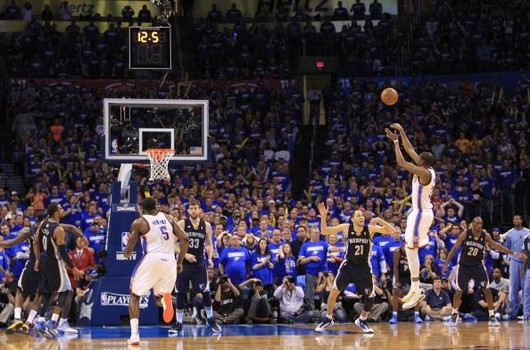
\includegraphics[width = 0.4\textwidth]{img/Triple.jpg}
\end{center}
\end{problem}

\begin{problem} Considera el $K$-homomorfismo $\appl{φ}{K[x,y]}{K[t]}$ con $φ(x) = t^2$ y $φ(t) = t^3$. Decide de manera razonada si φ factoriza por $\quot{K[x,y]}{\gen{x^2-y^2}}$. ¿Y por $\quot{K[x,y]}{\gen{x^3-y^2}}$?

\solution

\doneby{Guille} \inclass

Según se definía en la \fref{prop:FactorizacionHomomorfismo}, φ factoriza por $\quot{R}{I}$ si $I ⊂ \ker φ$, donde $\ker φ = \set{a ∈ R \tq φ(a) = 0}$. En el caso concreto de este ejercicio, lo que tenemos que ver es si $\gen{x^2 - y^2}$ y $\gen{x^3-y^2}$ están dentro de $\ker φ$.

Si $p(x,y) ∈ \gen{x^2-y^2}$, entonces $p(x,y) = a·(x^2-y^2)^n$ para $a ∈ K[x,y]$ y $n ∈ ℕ$. Calculando su imagen por $φ$, tenemos que \[ φ(p) = φ(a) · \left(φ(x^2) - φ(y^2)\right)^n = φ(a) · (t^4 - t^6)^n ≠ 0\], luego $\gen{x^2-y^2} \not\subset \ker φ$ y φ no factoriza por $\quot{K[x,y]}{\gen{x^2-y^2}}$.

Haciendo el proceso análogo con $p ∈ \quot{K[x,y]}{\gen{x^3-y^2}}$, nos saldrá que \[ φ(p) = φ(a) · (t^6 - t^6)^n = 0 \], así que $\gen{x^3-y^2} ⊂ \ker φ$ y $φ$ sí factoriza por $\quot{K[x,y]}{\gen{x^3-y^2}}$.

\end{problem}

\begin{problem}[6] \textbf{Teorema chino del resto}. Sea $R$ un anillo y sean $I_1, \dotsc, I_n$ ideales en $A$. Consideramos el siguiente homomorfismo de anillos:
\begin{align*}
\appl{φ}{R&}{\quot{R}{I_1} × \dotsb \quot{R}{I_n}} \\
r &\longmapsto (r_1, \dotsc, r_n)
\end{align*} donde $r_i$ denota la clase de $r$ módulo $I_i$. Demuestra que:

\ppart φ es sobreyectiva si y sólo si $I_i$ e $I_j$ son primos entre sí cuando $i ≠ j$.
\ppart φ es inyectiva si y sólo si $\bigcap I_i = \zerogen$.

\textit{Sugerencia general: Empieza considerando el caso $n = 2$. Para el primer apartado, en $\implies$ hay que observar que $(1,0)$ y $(0,1)$ tienen preimagen; para $\impliedby$ basta comprobar que $(1,0)$ y $(0,1)$ tienen preimagen. Para el segundo apartado, calcula $\ker φ$.}

\solution

\doneby{Guille}

Recordamos que dos ideales $I,J ⊂ R$ son \concept[Ideal\IS coprimo]{Ideales\IS coprimos} si $I + J = R$.

\spart

Demostrarmos primero la implicación a la derecha: si φ es sobreyectiva, entonces $I_i$ e $I_j$ son primos entre sí cuando $i ≠ j$. Vamos a demostrar que cualquier $a ∈ R$, con $a ∉ I_i, I_j$ se puede expresar como suma de elementos de $I_i$ e $I_j$.

Consideramos la imagen de $a$, $φ(a) = (a_1, \dotsc, a_n)$. Como $a$ no está ni en $I_i$ ni en $I_j$, tiene que ser $a_i, a_j ≠ 0$. Ahora bien, podemos descomponer $φ(a)$ como suma de tres elementos $φ(a) = α + a_i·1_i + a_j · 1_j$, donde $1_i$ es un vector nulo salvo por un $1$ en la coordenada $i$ y $α$ tiene las mismas coordenadas que $φ(a)$ salvo por la $i$-ésima y $j$-ésima, que son nulas.

Como φ es sobreyectiva, todos los sumandos tienen preimágenes. En concreto, la de $α$ está en $I_i ∩ I_j$, y las de $a_i · 1_i$ y $a_j · 1_j$ están en $I_j$ y en $I_i$ respectivamente. Por las propiedades de homomorfismo, la suma de esas preimágenes será igual a $a$, luego efectivamente cualquier $a ∉ I_i, I_j$ se puede expresar como suma de elementos de $I_i$ y $I_j$, por lo que $I_i$ e $I_j$ son primos entre sí.

Para la implicación al otro lado, suponemos que $I_i, I_j$ son coprimos cuando $i ≠ j$, y tratamos de demostrar que $φ$ es sobreyectiva. Como nos dice la sugerencia, nos basta con demostrar que $1_i$ tiene preimagen para $i = 1, \dotsc, n$, ya que sólo con eso podremos construir cualquier elemento en la imagen.

Si $φ(a) = 1_i$, significa que $a ∉ I_i$ pero $a ∈ I_j$ si $i ≠ j$. Si tal $a$ no existe, eso significa que cualquier elemento que esté en todos los $I_j$ con $i ≠ j$ está también en $I_i$. Luego $I_i ⊆ I_j$ para cualquier $j = 1, \dotsc, n$, contradicción porque entonces $I_j + I_j = I_j$ y no serían coprimos.

\spart

Sabemos que $a ∈ \ker φ \iff φ(a) = (0, \dotsc, 0)$, es decir, si y sólo si $a ∈ \bigcap I_i$. En otras palabras, $\ker φ = \bigcap I_i$, y efectivamente ya sabemos que φ es inyectiva si y sólo si $\ker φ = \zerogen$.

\end{problem}

\begin{problem} Demuestra que

\ppart Si $\gcd (n,m) = 1$ entonces $ℤ_{n·m} \simeq ℤ_n × ℤ_m$.
\ppart Demuestra que $\quot{ℝ[x]}{\gen{(x^2-1)x^3}}$ es isomorfo a la suma directa de tres anillos locales, que dos de ellos son un cuerpo y que el tercero tiene nilpotentes.

\solution

\inclass

\spart

Usamos el ejercicio anterior: si $R = ℤ_{nm}$, entonces hay dos ideales $I_1 = \gen{n}, I_2 = \gen{m}$ coprimos, y además $I_1 ∩ I_2 = \zerogen$. Por lo tanto, estamos en las condiciones del ejercicio anterior y el homomorfismo que se definía ahí $\appl{φ}{R}{\quot{R}{I_1} × \quot{R}{I_2}}$ es sobreyectivo e inyectivo, luego es isomorfismo y $ℤ_{n·m} \simeq ℤ_n × ℤ_m$.

\spart

De nuevo usando el ejercicio anterior, vemos que en el anillo $\quot{ℝ[x]}{\gen{(x^2-1)x^3}}$ hay tres ideales, $I_1 = \gen{x-1}$, $I_2 = \gen{x+1}$, $I_3 = \gen{x^3}$, por lo que es isomorfo \[ \quot{ℝ[x]}{\gen{(x^2-1)x^3}} \simeq \quot{ℝ[x]}{\gen{x-1}} × \quot{ℝ[x]}{\gen{x+1}} × \quot{ℝ[x]}{\gen{x^3}} \] donde $\quot{ℝ[x]}{\gen{x\pm 1}} \simeq ℝ$, que es un cuerpo, y en  $\quot{ℝ[x]}{\gen{x^3}}$ hay nilpotentes, tal y como nos pedían.

\end{problem}

\begin{problem} Encuentra ejemplos de anillos que verifiquen las siguientes condiciones:

\ppart Un anillo que tenga exactamente 2 ideales maximales y al menos un nilpotente no nulo.
\ppart Un anillo con un único ideal primo \pideal (por tanto necesariamente maximal) que no sea un cuerpo.

\solution

\inclass

\spart

Los ideales de $\quot{ℝ[x]}{\gen{x^3}}$ no son un misterio porque se corresponden de forma biyectiva con ideales de $ℝ[x]$ que contienen a $\gen{x^3}$. Sólo hay un maximal en $ℝ[x]$ que contenga a $\gen{x^3}$: $\gen{x}$.

Usando la misma idea, podemos coger $\gen{x^2(x-1)}$ que sólo tiene dos factores irreducibles ($x$ y $x-1$).

Otro ejemplo más fácil es $ℤ_{12}$.

\spart



\end{problem}

\begin{problem}[9] \label{ej:Hoja2:9} Demuestra que todo ideal $I \subsetneq R$ está contenido en un primo minimal siguiendo los siguientes pasos:

\begin{enumerate}
\item Considera el conjunto Σ de ideales primos de $R$ que contienen a $I$ y demuestra que no es vacío.
\item Define en Σ el siguiente orden parcial: $\mathfrak{p} ≤ \mathfrak{p}'$ si $\mathfrak{p}' ⊆ \mathfrak{p}$, y demuestra que toda cadena creciente de elementos en Σ tiene una cota superior en Σ.
\item Usa el \nref{lem:Zorn}.
\end{enumerate}

\solution

\spart


\end{problem}

\subsection{Problemas para entregar}

\begin{problem} Sea $R$ un anillo y sea $\mathfrak{p} ⊂ R$ un ideal primo. Demuestra que $\mathfrak{p}$ contiene un primo minimal, es decir, demuestra que existe un primo $\mathfrak{q} ⊂ \mathfrak{p}$ tal que si $\mathfrak{r} ⊂ R$ es otro ideal primo con $\mathfrak{r} ⊂ \mathfrak{q}$ entonces $\mathfrak{r} = \mathfrak{q}$.

\textup{Sugerencia: Puedes usar una idea parecida a la del \fref{ej:Hoja2:9}}.

\solution
\doneby{Parra}

Utilizaremos el Lema de Zorn: Sea $\Sigma$ un conjunto no vacío parcialmente ordenado. Si toda cadena creciente de elementos de $\Sigma$ tiene una cota superior, entonces $\Sigma$ tiene un elemento maximal.

Definimos el conjunto $\Sigma$ como el conjunto de todos los ideales primos contenidos en $p$, entonces:
\begin{itemize}
	\item $\Sigma \neq \emptyset$ ya que $\pideal \subset \pideal$.
	\item Definimos la siguiente relación: $\pideal \leq \pideal' \Leftrightarrow \pideal' \subset \pideal$.
	\item Sea $L=\{\pideal_i\}$ una cadena creciente de ideales primos, es decir $\pideal_n \leq \pideal_m\; \forall m \geq n$, que dada la relación de equivalencia definida es lo mismo que decir que $\pideal_n \supset \pideal_m\; \forall m \geq n$. Queremos ver que la cadena está acotada en $\Sigma$.

	Podemos coger como cota superior $\pideal_0=\bigcap_{\pideal_i\in L}$. Esta claro que $\pideal_0 \geq \pideal_i\; \forall i$, ya que $\pideal_0 \subset \pideal_i\;  \forall i$.

	Sabemos que la intersección de ideales es un ideal, por tanto, nos falta ver que $p_0$ es primo, es decir, que si tomamos $a,b \in R$ tal que $a\cdot b \in p_0$, entonces $a$ ó $b$ tiene que pertenecer a $\pideal_0$, es decir o $a$ o $b$ pertenecen a todos los $\pideal_i$ de L. Supongamos que no, tenemos dos posibilidades:
	\begin{enumerate}
		\item $a$ y $b$ no pertenecen a ningún $\pideal_i \in L$, entonces ningún $\pideal_i$ es primo, por lo que llegamos a contradicción.
		\item Suponemos que existen $a,b\in R$, tal que $a \in \pideal_i, b \notin \pideal_i$ y $a \notin \pideal_i,\, b \in \pideal_j$ con $j \neq i$. Que también nos llevaría a contradicción ya que, asumimos sin pérdida de generalidad que $\pideal_i \leq \pideal_j$, por tanto $\pideal_j \subset \pideal_i$, por tanto, $a,b \in \pideal_i$.
	\end{enumerate}

	Por tanto, tenemos cota superior, y cumplimos las hipótesis del Lema de Zorn. Lo aplicamos y tenemos que existe un elemento maximal, que es el primo minimal buscado.
\end{itemize}


\end{problem}


\begin{problem} Encuentra todos los primos minimales en

\ppart $ℤ_{12}$
\ppart $ℤ_9[x]$
\ppart $\quot{\K[x]}{\gen{x^3(x-1)}}$
\ppart $\quot{ℝ[x,y]}{\gen{x-y^2}}$.

\solution
\doneby{Parra}

\spart En $\ent_{12}$ tenemos 4 ideales distintos del total o del $\{\zero \}$ que son: $\gen{2}$, $\gen{3}$, $\gen{4}$ y $\gen{6}$. Los dos últimos no son primos ya que tenemos que $2 \cdot 2 \in \gen{4}$ y $2 \notin \gen{4}$. Y por otro lado $2 \cdot 3 \in \gen{6}$ y $2,3 \notin \gen{6}$.

Los únicos primos minimales son $\gen{2}$ y $\gen{3}$

\spart En $\ent_9[x]$ hacemos lo siguiente:

En primer lugar, sabemos que el $\zero$ pertenece a cualquier ideal, incluidos los ideales primos. En $Z_9[x]$ tenemos que $\zero=3\cdot 3$. Por tanto, el $3\in p$ para cualquier primo p. Por tanto $\gen{3} \subset p$ para cualquier primo p.

Ahora, vamos a ver qué es $\gen{3}$ en $\ent_9[x]$. Para ello definimos el anillo cociente:
$$ \quot{\ent_9[x]}{\gen{3}}\simeq\ent_3[x]$$

Pero $\ent_3[x]$ es un dominio de integridad (no es un cuerpo ya que el $x$ no tiene inverso, porque $\frac{1}{x} \notin \ent_3[x]$). Por ser dominio de integridad, entonces $\gen{3}$ es un ideal primo en $\ent_9[x]$.

Por tanto, $\gen{3}$ es el único primo minimal de $\ent_9[x]$

\spart

Queremos aplicar la idea de que sea un homomorfismo $f:R \longmapsto \quot{R}{I}$ tenemos que hay una correspondencia biyectiva entre los ideales primos en $R$ que contengan a $I$ y los ideales primos de $\quot{R}{I}$ (proposición \ref{prop:correspondencia_biyectiva}).

Por tanto tenemos que hay una correspondencia biyectiva entre los ideales primos en $\K[x]$ que contengan a $\gen{x^3(x-1)}$ y los ideales primos de $\quot{\K[x]}{\gen{x^3(x-1)}}$

\textbf{Dos formas parecidas de pensarlo:}
\begin{itemize}
	\item \textbf{Más para este ejemplo en particular:} En este caso, por ser $K$ un cuerpo, los ideales primos en $K[x]$ vienen dados por $\gen{p(x)}$ con $p(x)$ irreducible.

	Los dos únicos polinomios irreducibles que dividen a $x^3(x-1)$ son $x$ y $(x-1)$, por lo tanto, los dos únicos ideales primos que contienen a $\gen{x^3(x-1)}$ en $\K[x]$ son $\gen{x}$ y $\gen{x-1}$.

	Por la correspondencia biyectiva, los dos únicos ideales primos en $\quot{\K[x]}{\gen{x^3(x-1)}}$ son $\gen{x}$ y $\gen{x-1}$, que no se contienen entre ellos y por tanto son los dos primos minimales.

	\item \textbf{Más genérica:} vamos a coger los ideales primos $p \in R$ que contengan al ideal $\gen{x^3(x-1)}$.

	Por tanto, buscamos los ideales primos $p$ tal que el elemento $x^3(x-1) \in p$, entonces, por ser $p$ primo $x \in p$ o $(x-1) \in p$. Eso implica que  $\gen{x} \in p$ o $\gen{x-1} \in p$.

	Ahora vamos a ver qué tipo de ideales son $\gen{x}$ y $\gen{x-1}$

	En este caso, como hemos dicho antes, por ser $K$ un cuerpo, los ideales primos en $K[x]$ vienen dados por $\gen{p(x)}$ con $p(x)$ irreducible.

	En otros casos, para ver qué tipo de ideales definimos su anillo cociente:

	\begin{itemize}
		\item $\quot{K[x]}{\gen{x}} \simeq K$ que es un cuerpo, y por tanto un dominio de integridad. Por tanto $\gen{x}$ es primo y maximal.
		\item $\quot{K[x]}{\gen{x-1}}$.  Igual que el anterior.
	\end{itemize}

	Por tanto, tenemos que tanto $\gen{x}$ como $\gen{x-1}$ son primos en $K[x]$, y ambos contienen a $\gen{x^3(x-1)}$, entonces, por la correspondencia biyectiva. también son primos en $\quot{K[x]}{\gen{x^3(x-1)}}$. Así que $\gen{x}$ como $\gen{x-1}$ son los primos minimales de $\quot{K[x]}{\gen{x^3(x-1)}}$.
\end{itemize}

NOTA: Al ser $K$ un cuerpo, el ideal generado por un número, por ejemplo el $\gen{2}$, no es primo, ya que $2$ es una unidad.

\spart Puesto que $\cls{y}=\cls{x^2}$, entonces

 $$\quot{ℝ[x,y]}{\gen{x-y^2}} \simeq \real[y]$$

 Pero $\real[y]$ es un dominio de integridad, por tanto $\{0\}$ es ideal primo y por tanto $\{0\}$ es un ideal primo minimal.

\end{problem}

\begin{problem} Sea $\appl{f}{R}{T}$ un homomorfismo de anillos.

\ppart Demuestra que si $J ⊂ T$ es un ideal entonces $\inv{f}(J) = \set{r ∈ R \tq f(r) ∈ J}$ es un ideal en $ℝ$. Demuestra que necesariamente $\ker f  ⊂ \inv{f}(J)$.
\ppart Demuestra que si $I ⊂ R$ es un ideal, entonces $f(I) = \set{f(r) \tq r ∈ I}$ en general no es un ideal en $T$.
\ppart Demuestra que si $I ⊂ R$ es un ideal y $f$ es sobreyectiva entonces $f(I)$ es un ideal en $T$.

\ppart Sea $I ⊂ R$ un ideal. Aunque en general $f(I)$ no tiene por qué ser un ideal en $T$, podemos considerar el ideal que genera en $T$. Denotaremos por $I^e$ al ideal generado por $f(I)$ en $T$.  Demuestra que $I ⊂ \inv{f}(I^e)$ y que en general el contenido es estricto.
\ppart Sea $J ⊂ T$ un ideal. Demuestra que $(\inv{f}(J))^e ⊂ J$ y que en general el contenido es estricto.

\solution

\doneby{Guille}

\spart

Vamos a demostrar que es un ideal. Sabemos que no es vacío ya que $f(0) = 0$ y $0 ∈ J$ por ser ideal, luego $0 ∈ \inv{f}(J)$. La propiedad de absorción también se cumple: si $r ∈ R$ y $a ∈ \inv{f}(J)$, tenemos que $f(ra) = f(r)·f(a) ∈ J$ por la absorción de $J$, ya que $f(a) ∈ J$. Por último, queremos ver que si $a, b ∈ \inv{f}(J)$ entonces $a + b ∈ \inv{f}(J)$, que también se cumprueba fácilmente: $f(a+b) = f(a) + f(b) ∈ J$ por ser ser $J$ ideal.

Para la segunda proposición, si $a ∈ \ker f$ entonces $f(a) = 0 ∈ J$, por lo que $a ∈ \inv{f}(J)$.

\spart

Si tomamos la inclusión $\appl{i}{ℤ}{ℚ}$ e $I = \gen{2} ⊂ ℤ$, éste es un ideal en $ℤ$ pero $i(\gen{2}) ⊂ ℚ$ no lo es en $ℚ$, ya que no se cumpliría la propiedad de absorción.

\spart

Vamos a comprobarlo. Esta claro que $f(I)$ no será vacío si $I$ no lo es. Comprobamos la propiedad de absorción: sea $t ∈ T$ y $a ∈ f(I)$, con $a = f(b)$ y $b ∈ I$. Dado que $f$ es sobreyectiva, existe al menos un $r ∈ R$ tal que $f(r) = t$. Entonces podemos operar y ver que \[ t · a = f(r) · f(b) = f(r·b) ∈ f(I) \] ya que $r·b ∈ I$ por absorción de $I$.

Por último, queremos ver que si $a,b ∈ f(I)$, entonces $a+ b ∈ f(I)$. Denotamos $a = f(c), b = f(d)$ con $c,d ∈ I$ y entonces \[ a + b = f(c) + f(d) = f(c+d) ∈ f(I) \] ya que $c + d ∈ I$ igualmente.

\spart

Podemos ver que \[ \inv{f}(f(I)^e) = \set{r ∈ R \tq f(r) ∈ f(I)^e} \] o, en otras palabras, $r ∈ \inv{f}(f(I)^e)$ si y sólo si \[ f(r) = α_1 f(β_1) + \dotsb + α_n f(β_n)\] para unos ciertos $α_i ∈ T$ y $β_i ∈ I$. En concreto, si $r ∈ I$ simplemente podemos tomar $α_1 = 1 ∈ T$ y $β_1 = r ∈ I$, por lo que efectivamente $r ∈ I \implies r ∈ \inv{f}(f(I)^e)$.

Para demostrar que el contenido en general es estricto, vemos el ejemplo del apartado $B$: si tomamos la inclusión $\appl{i}{ℤ}{ℚ}$ e $I = \gen{2} ⊂ Z$, podemos ver que $3 = \frac{3}{2} · 2∈ f(I)^e$, pero $\inv{f}(3) = 3 ∉ \gen{2}$.

\spart

Por definición, $j ∈ (\inv{f}(J))^e$ si y sólo si existen unos ciertos $\set{t_i}_{i=1}^n ⊂ T$, $\set{r_i}_{i=1}^n ⊂ \inv{f}(J)$ tales que $j = t_1 f(r_1) + \dotsb + t_n f(r_n)$.

Ahora bien, $f(r_i) ∈ J$, por absorción sabremos que $t_i f(r_i) ∈ J$ y por lo tanto $j ∈ J$, así que efectivamente $(\inv{f}(J))^e ⊆ J$.

Para ver que el contenido en general es estricto... \noteby{Guille}{Ni idea de esto.}
\end{problem}

\begin{problem} Trabajamos en $ℝ[x,y]$. Sean $a,b ∈ ℝ$. ¿Cuál es la condición necesaria y suficiente para que un maximal de la forma $\gen{x-a, y-b}$ contenga al ideal $\gen{x-y^2}$?


\textup{Sugerencia: $\gen{x-y^2} ⊂ \gen{x-a, y-b}$ si y sólo si el homomorfismo del paso al cociente $ℝ[x,y] \mapsto \quot{ℝ[x,y]}{\gen{x-a, y-b}} \simeq ℝ$ factoriza por $\quot{ℝ[x,y]}{\gen{x-y^2}}$. ¿Por qué? Y ahora piensa, ¿cuál es el homomorfismo composición $ℝ[x,y] \mapsto ℝ$?}

\solution

\inclass

Una condición necesaria y suficiente para que $\gen{x-a, y-b} ⊂ K[x,y]$ sea maximal es que $K$ sea un cuerpo. Vamos ahora al ejercicio.

Lo primero es comprobar que $\gen{x-y^2}$ sea maximal. La respuesta es que no: $\quot{ℝ[x,y]}{x-y^2} \simeq ℝ[y]$, que no es un cuerpo luego $\gen{x-y^2}$ no es maximal. Lo que sí es es primo, ya que $ℝ[y]$ no tiene divisores de cero.

Una observación es ver que $\gen{x-y^2} ⊂ \gen{x-a, y-b}$ si y sólo si $\gen{x-a, y-b}$ es de los maximales de $ℝ[x,y]$ que están en correspondencia biyectiva con los maximales de $\quot{ℝ[x,y]}{\gen{x-y^2}}$. Ahora vamos a tratar de construir un $ℝ$-homomorfismo decidiendo a dónde mandamos a $x$ e $y$. En concreto, lo definiremos de la siguiente forma:
\begin{align*}
\appl{f}{ℝ[x,y]&}{ℝ} \\
x &\longmapsto a \\
y &\longmapsto b
\end{align*}

Aunque no lo pide el problema, podemos ver que $\ker f = \gen{x-a, y-b}$. El contenido obvio es que $\gen{x-a, y-b} ⊂ \ker f$, aunque para la inclusión al otro lado hay que pensar algo más. Como $\gen{x-a,y-b}$ es maximal, si $\ker f ≠ \gen{x-a, y-b}$ tendría que ser $\ker f = ℝ[x,y]$, pero eso no es un homomorfismo.

Volvemos otra vez al problema. Y tenemos que girar la ficha del puzzle o, en otras palabras tenemos que hacer que el diagrama de la \fref{fig:Teorema1Isomorfia:Diag1} conmute o, equivalentemente, que $f = f' ○ π$. Esto ocurrirá sólo si $a = b^2$, y esta es la condición que buscábamos

\begin{figure}
\centering
\begin{tikzpicture}[scale = 1.5]
\node (A) at (0,0) {$ℝ[x,y]$};
\node (B) at (4,0) {$\quot{ℝ[x,y]}{\gen{x-a,y-b}}$};
\node (C) at (2,-2) {$\quot{ℝ[x,y]}{\gen{x-y^2}}$};

\draw[->] (A) -- node[midway, above, align = center] {\footnotesize $x \to a$ \\ \footnotesize $y \to b$} node[midway, below] {$f$} (B);
\draw[->] (A) -- node[midway, below, sloped, align = center] {\footnotesize $x \to y^2$ \\ \footnotesize $y \to y$} node[midway, above, sloped] {$π$} (C);
\draw[->] (B) -- node[midway, below, sloped, align = center] {\footnotesize $y^2 \to a$ \\ \footnotesize $y \to b$} node[midway, above, sloped] {$f'$} (C);
\end{tikzpicture}
\caption{Diagrama que queremos hacer conmutativo}
\label{fig:EjHoja2:13}
\end{figure}

\end{problem}

\begin{problem} Demuestra que el ideal $\gen{x^2 + x - y} ⊂ ℝ[x,y]$ es primo. ¿Es maximal?

\solution

\doneby{Parra}

Tenemos que $\cls{x^2+x}= \cls{y}$.

Definimos la aplicación:
$$f:\real[x] \longmapsto \quot{ℝ[x,y]}{\gen{x^2+x-y}}$$

Es sobreyectiva ya que sea un $p(x,y) \in \real[x,y]$ cualquiera, se puede escribir como un $p(x) in \real[x]$.

Además también es inyectiva ya que $\ker(f)=\{p(x):\cls{p(x)}=0 \}$. Esos son los $p(x) \in \gen{x^2+x-y}$. Sea $p(x) \in \gen{x^2+x-y}$ en $\real[x,y]$, entonces $\exists q(x,y) \in \real[x,y]$ tal que $p(x)=q(x,y)(x^2+x-y)$. Lo cual solo es posible si $q(x,y)=0$, que implica que $p(x)=0$ y por tanto $\ker(f)=0$.

Así nos queda que:

$$\quot{ℝ[x,y]}{\gen{x^2+x-y}} \simeq \real[x]$$

Como $\real[x]$ es un dominio de integridad, entonces $\gen{x^2+x-y}$ es primo. Pero $\real[x]$ no es un cuerpo, ya que $x$ no tiene inverso multiplicativo porque $\frac{1}{x} \notin \real[x]$, por tanto, no es maximal.

\end{problem}

\section{Hoja 3: Módulos, localización}

\begin{problem} Sea $\appl{f}{R}{S}$ un homomorfismo de anillos y sea $N$ un $S$-módulo. Demuestra que, vía $f$, $N$ es de manera natural un $R$-módulo. En particular, observa que todo ideal de $S$ es un $R$-módulo, y que $S$ es un $R$-módulo.

\solution

\doneby{Guille}

La definición para que $N$ sea un $R$-módulo es clara: si φ es la operación externa $\appl{φ}{S×N}{N}$, entonces podemos definir otra operación externa para $N$ sobre $R$ de la siguiente forma: \begin{align*}
\appl{γ}{R × N&}{N} \\
(r,n) &\longmapsto φ(f(r), n)
\end{align*} cuyas propiedades sensatas se pueden calcular con facilidad, ya que van a venir dadas o bien porque las cumple φ o porque $f$ es homomorfismo. Vamos a ir una por una:

\begin{itemize}
\item $∀r ∈ R,\,∀n,n' ∈ N$ se cumple $γ(r, n + n') = φ(f(r), n + n') = φ(f(r), n) + φ(f(r), n') = γ(r,n) + γ(r,n')$, ya que $φ$ es la operación externa de $N$ como $S$-módulo.
\item $∀r,r' ∈ R,\, ∀n ∈ N$ tenemos que $γ(r+r',n) = φ(f(r+r'), n) = φ(f(r) + f(r'), n) = γ(r, n) + γ(r',n)$.
\item Del resto de propiedades ya paso porque salen igual, nos podemos hacer todos a la idea.
\end{itemize}

En clase habíamos visto que los ideales $I ⊂ S$ son $S$-módulos, por lo que dada la construcción que acabamos de hacer, también serán $R$-módulos. Como $S$ es un ideal de $S$, igualmente será un $R$-módulo.

\end{problem}

\begin{problem} Sea $R$ un anillo. Demuestra que $R[x_1, \dotsc, x_n]$ no es un $R$-módulo finitamente generado. Demuestra que en cambio es una $R$-álgebra finitamente generada. ¿Es $ℚ[\sqrt[3]{2}]$ una $ℚ$-álgebra finitamente generada? ¿Es $ℚ[\sqrt[3]{2}]$ un $ℚ$-módulo finitamente generado?

\solution

\end{problem}

\begin{problem} Sean $M$ y $N$ dos $R$-módulos.

\ppart Demustra que el conjunto de los homomorfismos de $R$-módulos de $M$ en $N$, $\mop{Hom}_R (M,N)$ es un $R$-módulo.

\ppart Considera la aplicación \begin{align*}
\appl{φ}{R&}{\mop{Hom}_R(M,M) = \mop{End}_R M} \\
r & \longmapsto f_r \end{align*} donde $f_r(m) = rm$. Demuestra que $φ$ es un homomorfismo de $R$-módulos, y que $\quot{R}{\mop{Ann}_R(M)} ⊂ \mop{End}_R(M)$, donde \[ \mop{Ann}_R(M) ≝ \set{a ∈ R \tq am = 0\;∀m ∈ M}\] es un ideal de $R$.

\solution

\doneby{Guille} \inclass

\spart

Por comodidad, voy a denotar $H = \mop{Hom}_R (M,N)$. La operación externa la vamos a definir de la siguiente forma: dados $r ∈ R$ y $f ∈ H$, entonces $(r,f) \mapsto r·f ∈ H$. Así, podemos verificar las propiedades:

\begin{itemize}
\item No es vacío: el homomorfismo $f(m) = 0$ que envía todo a cero siempre está en $H$.
\item $H$ es un grupo abeliano, ya que $(f+g)(m) = f(m) + g(m) = g(m) + f(m) = (g + f) (m)$.
\item $∀ r ∈ R,\,∀f,g ∈ H$ tenemos que ver cuánto vale $r · (f + g)$. Para calcularlo, aplicamos este homomorfismo a un elemento $m ∈ M$, y entonces \[ (r · (f+g))(m) = r · (f+g) (m) = r·f(m) + r·g(m) \], luego efectivamente se cumple si aceptamos que $(f+g)(m) = f(m) + g(m)$.
\item Análogamente.
\end{itemize}

Esto puede ser útil cuando tomamos $J,I ⊂ R$ ideales de $R$. Por ejemplo, si tomamos $r ∈ (I:J)$ (el conductor) tenemos $R$-homomorfismos. Lo interesante de este tipo de homomorfismo es algo. Otro caso curioso es cuando tenemos homomorfismos de $J$ en sí mismo, que puede ser una herramienta computacional para cosas.

\spart

La demostración de las propiedades de homomorfismo es trivial.

Para lo otro, vemos que $\ker φ = \set{r ∈ R \tq φ(r) = f_r = f_0}$, luego $\ker φ = \mop{Ann}_R (M)$. Entonces podemos usar los teoremas de isomorfía\footnoteby{Guille}{No estoy seguro de que se use esto.} y entonces hay una inclusión $\quot{R}{\mop{Ann}_R(M)} ⊂ \mop{End}_R(M)$.

\end{problem}

\begin{problem} Sea $I = \gen{\cls{2}} ⊂ ℤ_6$. Demuestra que $I$ es también un $ℤ_3$-módulo.

\solution

\inclass

Aplicamos lo que hemos visto en el ejercicio anterior, con $R = ℤ_6$ y $M = I$, y consideramos los endomorfismos $\mop{End}_{ℤ_6} (\gen{\cls{2}})$. Ahora calculamos y vemos que \[ \mop{Ann}_{ℤ_6} \gen{\cls{2}} = \gen{\cls{3}}\] y algo que me he perdido.

\end{problem}

\begin{problem}[11]

\solution

\spart

\spart

\textit{Comentario de Ana Bravo:}

\end{problem}


\subsection{Problemas para entregar}
\begin{problem}[1]
	Sea $M$ un $R$-módulo y sea $\mop{Ann}_R(M) ≝ \set{a \in R \tq  am = 0, \forall m \in M}$

	\ppart Demuestra que $\mop{Ann}_R(M)$ es un ideal

	\ppart Demuestra que $M$ tiene estructura de $R/\mop{Ann}_R(M)$-módulo y que ésta coincide con la que tiene como $R$-módulo.

	\ppart Considera el ideal $J = \gen{\cls{3}} \subset \ent_{12}$. Demuestra que $J$ es un $\ent_4$-módulo.

	\ppart Decide de manera razonada para qué valores de $n$, el ideal $J$ del apartado anterior es manera natural un $\ent_n$-módulo.

	\solution

	\spart
	\begin{itemize}
		\item $\mop{Ann}_R(M) \neq \emptyset$, ya que $0 \in \mop{Ann}_R(M)$, porque $0\cdot m = 0 \quad \forall m \in M$.
		\item Sea $a \in \mop{Ann}_R(M)$ y $b \in \mop{Ann}_R(M)$ entonces $a+b \in \mop{Ann}_R(M)$.

		Es cierto ya que si $am=0$ y $bm=0$ $\forall m \in M$, entonces por las propiedades sensatas de los $R$-módulos* podemos ver que $(a+b)m=am+bm=0+0=0$.
		\item Sea $a \in \mop{Ann}_R(M)$ y $r\in R$ entonces $(r\cdot a)m=0$ $\forall m \in M$.

		Cierto ya que si $a \in \mop{Ann}_R(M)$ entonces $am=0$, y por las propiedades sensatas de los $R$-módulos tenemos que:
		$r(r'm)=(rr')m \; \forall r,r' \in R, \; \forall m \in M$. Por tanto: $(ra)m=r(am)=r0=0$.
	\end{itemize}

	\spart

	Queremos ver primero que $M$ es un $\quot{R}{\mop{Ann}_R(M)}$-módulo:
	\begin{enumerate}
		\item $(M,+)$ es un grupo abeliano por ser $M$ un $R$-módulo.
		\item  Definimos la operación externa:
		\begin{align*}
			\quot{R}{\mop{Ann}_R(M)} × M & \longmapsto  M \\
			(\cls{r},m) & \longmapsto  \cls{r}\cdot m = rm \\
		\end{align*}
		Tenemos que ver que esta operacion está bien definida. Cogemos un representante de $\quot{R}{\mop{Ann}_R(M)}$, por ejemplo $\cls{r}=r+a$ con $a\in \mop{Ann}_R(M)$. Ahora definimos el producto:

		$$\cls{r} m = (r+a)m= rm+am \underbrace{=}_{a \in \mop{Ann}_R(M)} rm + 0 = rm$$

		Por tanto la operación no depende del representante escogido y la operación esta bien definida. Trivialmente se cumplen las propiedades sensatas.
	\end{enumerate}

	La estructura de $R$-módulo se define la operación externa de la misma forma:

	\begin{align*}
		R × M & \longmapsto  M \\
		(r,m) & \longmapsto  r\cdot m = rm \\
	\end{align*}

	Por tanto $M$ tiene estructura de  $\quot{R}{\mop{Ann}_R(M)}$-módulo y también de $R$-módulo, y estas coinciden. \textcolor{blue}{Las propiedades romanas se cumplen tanto para $M$ como para el cociente, por lo cumplen para $M$ como $R$-módulo. No hace falta probarlo pero hay que decirlo.}

	\spart

	\textcolor{blue}{Basta observar que $\mop{Ann}_{ℤ_{12}} J = \gen{4}$, luego $\quot{\quot{ℤ}{12}}{\quot{4}{12}} \simeq ℤ_4$.} ¿?

	Vamos a probar las dos propiedades:
	\begin{itemize}
		\item $(J,+)$ es un grupo abeliano. Cierto.
		\item  Sea $J=\gen{\cls{3}}=\{ \cls{0}, \cls{3}, \cls{6}, \cls{9} \}$. Definimos la operación externa:
		\begin{align*}
		\ent_4 × J & \longmapsto  J \\
		(\cls{a},\cls{m}) & \longmapsto  \cls{a}\cdot \cls{m} =\cls{a\cdot m} \\
		\end{align*}

		Vamos a ver que este producto está bien definido, es decir, que no depende de los representantes escogidos: $\cls{a}=a+4l$, y $\cls{m}=3n+12k$. Operamos:
		$$\cls{a}\cdot \cls{m}=a3n+12ak+12ln+48lk \eqreasonup[\equiv]{$\mod 12$} a3n=\cls{a3n}=\cls{a}\cls{3n}$$

		Vemos que efectivamente esta operación no depende de los representantes obtenidos y por tanto está bien definida.

		Las propiedades sensatas se cumplen trivialmente \textcolor{blue}{porque se cumplen para $J$ como $ℤ_{12}$-módulo y la estructura de $ℤ_4$-módulo la hereda. También se puede usar el apartado anterior: $\mop{Ann}_{ℤ_{12}} = \gen{\cls{4}}$, luego es un $ℤ_4$-módulo.}
	\end{itemize}

	\spart Para $n=4t \quad \forall t \in \nat$.

	\begin{align*}
	\ent_{4t} × J & \longmapsto  J \\
	(\cls{a},\cls{m}) & \longmapsto  \cls{a}\cdot \cls{m} =\cls{a\cdot m} \\
	\end{align*}

	Vamos a ver que este producto está bien definido, es decir, que no depende de los representantes escogidos: $\cls{a}=a+4tl$, y $\cls{m}=3n+12k$. Operamos:
	$$\cls{a}\cdot \cls{m}=a3n+12ak+12tln+48tlk \underbrace{\equiv}_{mod 12} a3n=\cls{a3n}=\cls{a}\cls{3n}$$

\end{problem}

\begin{problem}
	Sea $R=K[x,y]/\gen{xy}$ y sea $\appl{f}{R}{R_{\gen{x}}}$ el homomorfismo de paso al localizado.

	\ppart Describe $S =R \setminus \gen{x}$

	\ppart A la vista del apartado anterior, ¿qué elementos $a \in R$ serán invertibles vía $f$?

	\ppart Calcula $\ker f$.

	\ppart Utiliza los apartados anteriores y la propiedad universal de la localización para demostrar que ${R_{\gen{x}} \simeq K(y)}$.

	\solution

	\spart

	$R \setminus \gen{x}$ son los elementos de $R$ que no son múltiplos de $x$.

	\spart

	Los elementos invertibles será los $p(x,y) ∈ R\setminus \gen{x}$, es decir, los polinomios que no son múltiplos de $x$.

	\spart

	Sabemos que, dado $a ∈ R$, $f(a) = 0 \iff ∃s ∈ S \setminus \gen{x}$ tal que $s · a = 0$. Si $a ∈ \gen{x}$, entonces podemos encontrar un polinomio $p ∈ S$ con variables sólo en $y$ de tal forma que $a·p ∈ \gen{xy}$. Por otra parte, si $a ∉ \gen{x}$, entonces no es múltiplo de $x$, y si lo multiplicamos por cualquier elemento $s ∈ S$ $a·s$ no va a ser divisible por $xy$, ya que ni $a$ ni $s$ lo son.

	En definitiva, $\ker f = \gen{x}$.

	\spart

\end{problem}

\begin{problem}
	Sea $R$ un anillo, sea $I \subset R$ un ideal y sea $S \subset R$ un subconjunto multiplicativamente cerrado. Considera el homomorfismo de paso al cociente $\appl{\pi}{R}{R/I}$.

	\ppart Demuestra que $\pi(S)$ es un conjunto multiplicativamente cerrado en $R/I$.

	\ppart Demuestra que da lo mismo primero localizar y después cocientar, que primero cocientar y luego localizar. Es decir, demuestra que $S^{-1}R/IS^{-1}R \simeq \pi(S)^{-1}(R/I)$.

	\textit{Sugerencia: considera el siguiente diagrama y utiliza la la propiedad universal para probar que hay un homomorfismo (sobreyectivo) de $S^{-1}R$ en $\pi(S)^{-1}(R/I)$ de modo que el diagrama conmute. Y ahora usa el Primer Teorema de Isomorfía.}

	% http://tex.stackexchange.com/questions/45741/commutative-diagrams-and-tikz
	\begin{large}
	\begin{center}
	\begin{tikzpicture}
	    % set up the nodes
	    \node (R) at (0,0) {$R$};
	    \node[right=of R] (RI) {$R/I$};
	    \node[below=of RI] (SR) {$S^{-1}R$};
	    \node[right=of RI] (piSRI) {$\pi(S)^{-1}(R/I)$};
	    % draw arrows and text between them
	    \draw[->] (R)--(RI) node [midway,above] {$\pi$};
	    \draw[->] (R)--(SR) node [midway,below,sloped] {$f$};
	    \draw[->] (RI)-- node[midway, above] {$γ$} (piSRI);
	    \draw[->] (R) to[bend left=45] node[midway, above] {$φ$} (piSRI.north west);

	    \draw[->] (SR) --node[midway, below, sloped] {$g$} (piSRI.south west);
	\end{tikzpicture}
	\end{center}
	\end{large}

	\ppart Demuestra de otro modo el resultado obtenido en 2c, ahora usando el apartado 3b.

	\textit{Sugerencia: puede que te resulte útil el ejercicio 8.}

	\solution

	\spart

	Para ver que $\cls{1} ∈ π(S)$, simplemente hay que ver que $1 ∈ S$ por ser éste parte mulitplicativa, y entonces $π(1) = \cls{1} ∈ π(S)$.

	Sólo falta ver que dados $\cls{s}, \cls{s'} ∈ π(S)$, entonces $\cls{s}·\cls{s'} ∈ π(S)$. Pero $\cls{s}·\cls{s'} = \cls{s·s'}$, y como $S$ es parte multiplicativa, $ss' ∈ S$, y además ha de ser $π(ss') = \cls{s·s'}$, por lo que efectivamente es conjunto multiplicativamente cerrado.

	\spart

	La propiedad universal de la localización nos dice que si $\appl{φ}{R}{B}$ es un homomorfismo de anillos que lleva elementos de $S ⊂ R$ a unidades en $B$, entonces existe un único homomorfismo de anillos $\appl{g}{S^{-1}R}{B}$ tal que $φ = g ○ f$, con $f$ el homomorfismo de paso al localizado $f(a) = \frac{a}{1}$.

	En nuestro caso, si $\appl{γ}{\quot{R}{I}}{\pi(S)^{-1}(R/I)}$ es el homomorfismo de paso al localizado $\pi(S)^{-1}(R/I)$, entonces la aplicación $\appl{φ = γ ○ π}{R}{\pi(S)^{-1}(R/I)}$ es un homomorfismo de anillos por ser composición de homomorfismos. Vamos a comprobar qué ocurre con los elementos de $s$.

	Si $s ∈ S$, entonces $φ(s) = \frac{\cls{s}}{1}$. Queremos ver que su inverso, que debería ser el elemento $\frac{1}{\cls{s}}$, existe en $π(S)^{-1} (\quot{R}{I})$. Pero el localizado se construye como $\quot{R}{I} × π(S)$ con una relación de equivalencia, y está claro que $\cls{1} ⊂ \quot{R}{I}$ y $\cls{s} ∈ π(S)$, luego $φ(s)$ es invertible.

	Así, podemos aplicar la propiedad universal y ver que existe un único homomorfismo de anillos $\appl{g}{S^{-1}R}{\pi(S)^{-1}(R/I)}$ que hace conmutar el diagrama.

	Tenemos que demostrar que $g$ es sobreyectivo. Afirmamos que la preimagen de un elemento $\frac{\cls{r}}{\cls{s}}$ es $\frac{r}{s}$, y vamos a demostrarlo. Lo primero es ver que $\frac{r}{s} = \frac{r}{1} · \frac{1}{s}$, y como $g$ es homomorfismo podemos simplemente sacar las preimágenes por separado.

	Consideramos $r ∈ R$. Entonces tenemos que \begin{align*}
	(γ ○ π) (r) &= (g○f)(r) \\
	γ(π(r)) &= g(f(r)) \\
	γ(\cls{r}) &= g\left(\frac{r}{1}\right) \\
	\frac{\cls{r}}{\cls{1}} &= g\left(\frac{r}{1}\right)
	\end{align*} así que, tal y como necesitábamos, $g(\frac{r}{1}) = \frac{\cls{r}}{\cls{1}}$. Ahora nos falta ver el análogo para elementos de la forma $\frac{1}{s}$.

	En este caso simplemente tenemos que operar y ver que, por ser $g$ homomorfismo de anillos, \[ \frac{\cls{1}}{\cls{1}} = g\left(\frac{1}{1}\right) = g\left(\frac{s}{1}·\frac{1}{s}\right) = g\left(\frac{s}{1}\right) · g\left(\frac{1}{s}\right) = \frac{\cls{s}}{\cls{1}} · g\left(\frac{1}{s}\right)  \]

	Dado que el inverso es único, $g(\frac{1}{s})$ sólo puede ser $\frac{\cls{1}}{\cls{s}}$. Con esto vemos que \( g\left(\frac{r}{s}\right) = g\left(\frac{r}{1}·\frac{1}{s}\right) = \frac{\cls{r}}{\cls{1}} · \frac{\cls{1}}{\cls{s}} = \frac{\cls{r}}{\cls{s}} \label{eq:H3:DefHomoG} \)

	Esto nos permite dar la preimagen de cualquier $\frac{\cls{r}}{\cls{s}} ∈ \pi(S)^{-1}(R/I)$, luego $g$ es sobreyectiva.

	Ahora afirmamos que $\ker g = IS^{-1}R$, es decir, el ideal generado por $f(I) ⊂ \inv{S}R$. La idea es que si tenemos un elemento $\frac{r}{1} ∈ f(I)$, con $r ∈ I$, éste va a ser preimagen por $f$ de $r ∈ I ⊂ R$. Yendo por el otro lado del diagrama, vemos que $π(r) = 0$ y por lo tanto $φ(r) = \cls{0} ∈ π(S)^{-1} \quot{R}{I}$. Así, la única posibilidad es que $g(\frac{r}{1}) = \cls{0} ∈ π(S)^{-1}$. Por las propiedades de homomorfismos, los elementos de $f(I)^e$ estarán igualmente en $\ker g$.

	Por otra parte, tenemos que ver que si $\frac{r}{s} ∉ IS^{-1}R$ entonces $g(\frac{r}{s}) ≠ 0$. Pero teniendo en cuenta la definición de $g$ de \eqref{eq:H3:DefHomoG}, la única forma es que $r ∈ I$, luego $\frac{r}{s} ∈ IS^{-1}R$, contradicción.

	Finalmente, aplicamos el primer teorema de isomorfía y nos queda lo que queríamos demostrar:
	\begin{align*}
	\quot{S^{-1}R}{\ker g} &\simeq \img g \\
	\quot{S^{-1}R}{IS^{-1}R} &\simeq \pi(S)^{-1}(R/I)
	\end{align*}

	\spart

\end{problem}



\begin{problem}
	Sean $\mathfrak{q}\subset \mathfrak{p}$ dos ideales primos. Demuestra que los ideales primos de $R_\mathfrak{p}/\mathfrak{q}R_\mathfrak{p}$ están en correspondencia biyectiva con los ideales de $R$ que están contenidos en $\mathfrak{p}$ y que contienen a $\mathfrak{q}$.


	\solution

	Escribimos cada elemento para entender mejor el problema:

	$R_p = \{S^{-1}R $ con $ S=R \setminus p \} = \{\frac{r}{s}$, $r \in R$, $s \in R\setminus p \}$ , es decir, hacemos invertibles los elementos de $p$ complementario.

	$qR_p = \{ \varphi(q)^e\subset R_p$ con $\varphi : R \rightarrow S^{-1}R\} = \{\frac{r}{s} \in R_p$ tales que $\frac{r}{s} = \sum^N_{i=0} \frac{r'_i}{s'_i} \frac{q_i}{1}$, $q_i\in q$, $\frac{r'_i}{s'_i}\in R_p\}$

	Es claro que $qR_p \subset R_p$ y por tanto $R_p/qR_p$ será el conjunto que elimina las fracciones cuyos numeradores son generados por $q$.

	Hemos visto en teoría que los ideales del paso al localizado ($\varphi$) quedan invariantes (correspondencia biyectiva) a menos que tengan elementos comunes con $S$, si un ideal contiene un elemento en $S$, al pasar al localizado este elemento se vuelve invertible y por tanto unidad, con lo que la imagen por $\varphi$ extendida será el total ($\varphi(S)^e = S^{-1}R$). También vimos que ideales primos en $R$ van a parar al ideal generado por su imagen en $S^{-1}R$ que también son primos.

	Utilizando el ejercicio anterior construimos el siguiente diagrama:

	\begin{tikzpicture}
	\node (R) at (0,0) {$R$};
	\node (Rq) at (2,1) {$\quot{R}{\mathfrak{q}}$};
	\node (Rp) at (2,-1) {$\inv{S}R$};
	\node (supadre) at (4,0) {$\quot{R_\mathfrak{p}}{\mathfrak{q}R_\mathfrak{p}}$};

	\draw[->] (R) -- node[midway, above] {$π$} (Rq);
	\draw[->] (Rq) -- node[midway, above] {$φ'$} (supadre);
	\draw[->] (R) -- node[midway, above] {$φ$} (Rp);
	\draw[->] (Rp) -- node[midway, above] {$π'$} (supadre) ;
	\end{tikzpicture}

	Y hemos demostrado que el núcleo del paso al cociente ($\pi '$) es la imagen de $q$ por $\varphi$ extendida. Entonces hay correspondencia biyectiva entre los ideales primos de $S^{-1}R$ que contienen a $q$ y los ideales primos de $R_p/qR_p$ y además hay corespondencia biyectiva entre los ideales primos de $R$ que contienen a $q$ (contenidos ya en $p$) y los ideales primos de $S^{-1}R$

\end{problem}

\section{Hoja 4: Anillos noetherianos}

\subsection{Ejercicios para entregar}


\begin{problem}[1]
	Sea $R$ un anillo en el que todo ideal primo es finitamente generado. Demuestra que $R$ es noetheriano siguiendo los siguientes pasos. En primer lugar considera el conjunto de ideales:

	$$\Sigma = \{ I \subset R: I \text{ no es finitamente generado } \}.$$
	\ppart Si suponemos $\Sigma \neq \emptyset$, demuestra que tiene un elemento maximal digamos $\pideal$.
	\ppart Demuestra que $\pideal$ es un ideal primo del siguiente modo:
		\begin{enumerate}
			\item Si $x \notin \pideal$ demuestra que el ideal $\pideal+\gen{x}$ es finitamente generado; si además $Y \notin \pideal$ pero $xy \in \pideal$ demuestra que el ideal $(\pideal: \gen{x})$ es finitamente generado.
			\item Demuestra que existe un ideal finitamente generado $\aideal \subset \pideal$ tal que $\aideal + \gen{x}=\pideal + \gen{x}$. \textit{Sugerencia: Como $\pideal+\gen{x}$ es finitamente generado existen $\alpha_1,...,\alpha_s \in \pideal + \gen{x}$ tales que $\gen{\alpha_1,...,\alpha_s}=\pideal + \gen{x}$; ahora para cada i, $\alpha_i=a_i+b_ix$, con $a_i \in \pideal$, y $b_i \in R$...}
			\item Demuestra que para el ideal $\aideal$ del apartado anterior se tiene que $\aideal+x(\pideal:\gen{x})$. \textit{Sugerencia: Utiliza la igualdad del apartado
			anterior.}
		\end{enumerate}
	\ppart Concluye que R es noetheriano.


	$$\Sigma = \{ I \subset R: I \text{ no es finitamente generado } \}.$$
	\ppart Si suponemos $\Sigma \neq \emptyset$, demuestra que tiene un elemento maximal digamos $\pideal$.
	\ppart Demuestra que $\pideal$ es un ideal primo del siguiente modo:
	\begin{enumerate}
		\item Si $x \notin \pideal$ demuestra que el ideal $\pideal+\gen{x}$ es finitamente generado; si además $Y \notin \pideal$ pero $xy \in \pideal$ demuestra que el ideal $(\pideal: \gen{x})$ es finitamente generado.
		\item Demuestra que existe un ideal finitamente generado $\aideal \subset \pideal$ tal que $\aideal + \gen{x}=\pideal + \gen{x}$. \textit{Sugerencia: Como $\pideal+\gen{x}$ es finitamente generado existen $\alpha_1,...,\alpha_s \in \pideal + \gen{x}$ tales que $\gen{\alpha_1,...,\alpha_s}=\pideal + \gen{x}$; ahora para cada i, $\alpha_i=a_i+b_ix$, con $a_i \in \pideal$, y $b_i \in R$...}
		\item Demuestra que para el ideal $\aideal$ del apartado anterior se tiene que $\aideal+x(\pideal:\gen{x})$. \textit{Sugerencia: Utiliza la igualdad del apartado
			anterior.}
	\end{enumerate}
	\ppart Concluye que R es noetheriano.

	\solution

	\spart

	Vamos a utilizar el Lema de Zorn
	\begin{lemma}[Lema de Zorn]
		Sea $\Sigma$ un conjunto no vacío parcialmente ordenado. Si toda cadena creciente de elementos de $\Sigma$ tiene una cota superior, entonces $\Sigma$ tiene un elemento maximal.
	\end{lemma}

	Si suponemos que $\Sigma \neq \emptyset$ entonces podemos aplicar el Lema de Zorn ya que:
	\begin{itemize}
		\item $\Sigma \neq 0$ por suposición
		\item $\Sigma$ está parcialmente ordenado con la inclusión de ideales.
		\item Si $\{ J_n\}$ es una cadena creciente de ideales ($J_n \subset J_m$ $\forall m\geq n$), vamos a comprobar que la cadena está acotada en $\Sigma$.
	\end{itemize}
	Sea $\pideal = \bigcup J_n$. Queremos ver que $H \in \Sigma$, es decir, que es un ideal y que $\pideal$ no es finitamente generado.
	Si así lo fuese está claro que $\pideal$ sería una cota superior (contiene a todos los $J \in \Sigma$) y podríamos aplicar el Lema de Zorn para decir que $\Sigma$ tiene un elemento maximal.

	Esta claro que no es finitamente generado ya que es la unión de ideales y todos ello no son finitamente generados. Vemos que es un ideal:
	\begin{itemize}
		\item $\pideal \neq \emptyset$ ya que $0 \in J_n \forall n$, ya que el ideal más pequeño de todos es el $\set{0}$, además el elemento \zero pertenece a todos los ideales. Por tanto $\zero \in H$.
		\item Sean $a,b \in \pideal=\bigcup J_n$.  Entonces $\exists m,k \in \nat$ tal que $a \in J_m$ y $b \in J_k$. Sin pérdida de generalidad supongamos que $m \geq k$. Entonces $a,b \in J_m$, y por tanto $a+b \in J_m \subset \pideal$.
		\item Si $r\in R$ y $a \in \pideal$, entonces $ra \in H$. Cierto porque $a \in J_i$ para algún i, y $J_i$ es un ideal.
	\end{itemize}

	Aplicamos el Lema de Zorn y tenemos que $\pideal$ es un elemento maximal de $\Sigma$

	\spart

	\textbf{i):} Puesto que $\pideal$ es maximal de $\Sigma$, cualquier ideal no finitamente generado está contenido en $\pideal$.

	Por tanto si $x \notin \pideal \implies \gen{x} \not\subset \pideal \implies \pideal+\gen{x}  \not\subset \pideal \implies \pideal+\gen{x}$ es finitamente generado.

	En cuanto a lo otro, tenemos que:
	$$(\pideal:\gen{x})=\{a \in R : a\gen{x} \subset \pideal \}$$

	$y \in R, \; y \notin \pideal, \; xy \in \pideal \implies y\gen{x} \subset \pideal \implies y \in (\pideal:\gen{x}) \implies (\pideal:\gen{x})$ es finitamente generado (por contener a un elemento que no pertenece a $\pideal$).

	\textbf{ii):}

	$$\pideal + \gen{x} = \{ a + bx: a \in \pideal, b \in R \} $$

	Puesto que $\pideal + \gen{x}$ es finitamente generado, entonces existen $\alpha_1,...,\alpha_s \in \pideal + \gen{x}$ tales que $\pideal + \gen{x} = \gen{\alpha_1,...,\alpha_s}$. Por tanto, para cada $i, \alpha_i=a_i +b_ix$ con $a_i \in \pideal$ y $b_i \in R$.

	Cogemos $\aideal = \gen{a_1,...,a_s}$ y nos queda:

	Vamos a ver que si $c \in \pideal + \gen{x} \implies c \in \aideal + \gen{x}$. Esto es obvio ya que $c = a_i+b_ix$ para algún con $a_i \in \pideal$ y $b_i \in R$. Y $a_i \in \aideal$.

	Ahora vemos la otra inclusión: si $c \in \aideal + \gen{x} \implies c \in \pideal + \gen{x}$. En este caso $c = d_ia_i+b_ix$ para algún con $a_i \in \aideal$ y $b_i, d_i \in R$. Tenemos que $d_ia_i \in \aideal \subset \pideal \implies d_ia_i \in \pideal \implies c \in \pideal + \gen{x}$.

	\textbf{iii):}

	En el apartado anterior hemos visto que con $x \notin \pideal$ se cumple que $\aideal+\gen{x}=\pideal +\gen{x}$.

	Además, también hemos visto que $(\pideal:\gen{x})$ es finitamente generado. Por tanto $x(\pideal:\gen{x})$ es finitamente generado. Por tanto aplicando la igualdad anterior:

	$$\aideal + x(\pideal: \gen{x}) = \pideal + x(\pideal: \gen{x})$$

	Pero $\pideal + x(\pideal: \gen{x}) = \{ a+xb : a\in \pideal,  b \gen{x} \subset \pideal \} = \{ a+xb : a\in \pideal,  xb \in \pideal \} = \pideal$

	\spart

	Por tanto hemos probado que $\pideal$ es finitamente generado, y por lo tanto primo, con lo cual llegamos a contradicción $\implies$ $\Sigma = \emptyset \implies$ todo ideal en R es finitamente generado, que es la definición de anillo noetheriano.
\end{problem}

\begin{problem}[2]
	Sea $\K$ un cuerpo y sea $R=\prod_{i=1}^{\infty} \K$.
	\ppart Demuestra que $R$ no es un anillo noetheriano.
	\ppart Para cada $i=1,2,...$, considera el homomorfismo proyección en la i-ésima coordenada $\pi_i:R \rightarrow \K$. Describe $\ker(\pi_i)$. ¿Es un ideal primo?.
	\ppart Sea $\pideal \subset R$ un ideal primo, y para cada $i=1,2,..$ sea $e_i \in R$ el elemento que tiene 1 en la i-ésima coordenada y 0 en el resto. Supongamos que $e_i \notin \pideal$. Demuestra que $e_1e_i \in \pideal$ para todo $i \geq 2$. ¿Qué concluyes?
	\ppart Utiliza los apartados anteriores para demostrar que $R$ tiene infinitos primos minimales.

	\solution

	\spart
	$R=  \prod_{i=1}^{\infty} \K = \K \times \K \underbrace{\times... \times}_{\infty \text{ veces}} \K$

	$R$ tiene por tanto infinitas coordenadas, es decir, un elemento de R es de la forma $\cls{x}=\{x_1,x_2,...,x_n,...\}$.

	Definimos una cadena creciente de ideales $\{I_i\}_{i \in [0,\infty)}$ tal que $I_i = \underbrace{\K \times... \times \K}_{i\text{ veces}} \underbrace{\times 0 \times ...  \times 0}_{\infty \text{ veces}}$. Vemos que $I_i$ nunca estabiliza.

	Por tanto R no es noetheriano.


	\spart

	Definimos $\ker(\pi_i)$:
	$$ \ker(\pi_i)=\{ a \in R: \pi_i(a)=0 \} $$

	Como $\K$ es un cuerpo, no tiene divisores de 0, por tanto, $\ker(\pi_i) = \{ a \in R: a_i=0 \}$ es decir, los elementos de R que tienen un 0 en su i-ésima coordenada.

	Basándonos en el primer teorema de isomorfía tenemos que:
	$$\quot{R}{\ker(\pi_i)} \simeq \img(\pi_i)$$


	Puesto que  $\img(\pi_i)$ es un ideal de $\K$ cuerpo, entonces $\img(\pi_i)$ es un cuerpo y por tanto $\ker(\pi_i)$ es primo.

	\spart

	Está claro que $e_1e_i = 0, \; \forall i \geq 2$. Y el 0 pertenece a cualquier ideal, por tanto $e_1e_i \in \pideal$ Concluyo entonces que $e_i \in \pideal \; \forall i \geq 2$ y que $\pideal = \{0\} \times \K \times \K \underbrace{\times... \times}_{\infty \text{ veces}} \K$

	\spart

	Sea $\pideal_i =  \K \times ... \times \K \times \underbrace{\{0\}}_{i} \times \K \times ... \times \K$

	Como hemos visto en el apartado anterior $\pideal_i$ es primo $\forall i$. Si demostramos que es primo minimal, ya habríamos demostrado que tenemos infinitos primos minimales.

	Puesto que $\K$ es un cuerpo, sus únicos ideales son $\{0\}$ y $\K$. Sea:

	$\pideal_{ij} =  \K \times ... \times \K \times \underbrace{\{0\}}_{i} \times \K \times ... \times \K \times \underbrace{\{0\}}_{j} \times \K \times ... \times \K$

	Para dos posiciones $i$ y $j$ cualesquiera, entonces $\pideal_{ij}$ no es primo ya que $e_j, e_i \notin \pideal_{ij}$ y $e_je_i=0 \in \pideal_{ij}$. Lo mismo ocurre si en lugar de dos $\{0\}$ hay 3 o más. Por tanto, no existe ningún otro ideal primo que esté contenido en $\pideal_i \implies$ es primo minimal $\implies$ tenemos infinitos ideales primos minimales.
\end{problem}

\begin{problem}[3] Sea $D$ un dominio de ideales principales.

	\ppart Demuestra que dos ideales $\gen{a}, \gen{b} ⊂ D$ son iguales si y sólo si existe una unidad $u ∈ D$ tal que $a = ud$, es decir, en un DIP dos elementos generan el mismo ideal si y sólo si son asociados.

	\ppart Demuestra que un ideal $\mathfrak{m} ⊂ D$ es maximal si y sólo si está generado por un elemento irreducible.

	\ppart Demuestra que todo elemento irreducible $a ∈ D$ es primo.

	\solution

	\spart

	Si $\gen{a} = \gen{b}$, entonces $a = r_1 b$ y $b = r_2 a$, luego $a = r_1 r_2 a$. Así, $r_1 r_2 = 1$, de tal forma que $r_1, r_2$ son unidades y entonces $a$ y $b$ son asociados.

	Si $a = ub$ con $u ∈ D$ unidad, entonces $∀c ∈ \gen{a}$ tenemos que $c = r · a = ru b$, luego $c ∈ \gen{b}$. Análogamente y sabiendo que $b = \inv{u} a$ se demuestra que todo $c ∈ \gen{b}$ está también en $\gen{a}$ y entonces ambos ideales son iguales.

	\spart

	Si $\mathfrak{m}$ no es maximal, entonces existe otro ideal $I ⊂ D$ tal que $\mathfrak{m} \subsetneq I$. Por ser $D$ un DIP, entonces existen $a,b ∈ D$ tales que $\mathfrak{m} = \gen{a}$ y $I = \gen{b}$. Como $\mathfrak{m} ⊂ I$, entonces $a = cb$ con $c ∈ D$. Además, $c$ no puede ser una unidad porque entonces $a$ y $b$ serían asociados y generarían el mismo ideal. Por lo tanto, $a$ no es irreducible.

	Si por el contrario $\mathfrak{m} = \gen{a}$ es maximal, entonces tenemos que demostrar que si $a = bc$ para $b,c ∈ D$, entonces $b$ ó $c$ son una unidad. Supongamos que no fuese así y ninguno es unidad. Entonces $a ∈ \gen{c}$ y por lo tanto $\gen{a} ⊆ \gen{c}$. Pero $\gen{a}$ es maximal, luego $\gen{a} = \gen{c}$, y por el apartado anterior $a$ y $c$ han de ser asociados, de tal forma que en la descomposición $a = bc$, $b$ debería de ser una unidad, contradicción. Luego si $\gen{a}$ es maximal, entonces $a$ es irreducible.

	\spart

	Si consideramos el ideal $\gen{a}$, es maximal por el apartado anterior, y dado que todo ideal maximal es primo, entonces $a$ es primo.

\end{problem}

\begin{problem}[4] \textbf{Dominios de factorización única (DFU)} Un dominio de integridad $D$ es un dominio de factorización única (DFU) si cada elemento no nulo de $D$ se puede escribir como producto de un número finito de irreducibles de manera única, salvo orden o producto por unidades.

	\ppart Demuestra que todo dominio de ideales principales $D$ es un dominio de factorización única. \textit{Sugerencia: sea $a ∈ D$ no nulo y no invertible. Si $a$ no es irreducible, entonces $a = a_1 b_1$ con $b_1$ irreducible. ¿Por qué? Si $a_1$ no es irreducible, entonces $a_1 = a_2 b_2$ con $b_2$ irreducible, e iterando tendríamos una cadena creciente de ideales $\gen{a} ⊂ \gen{a_1} ⊂ \gen{a_2} ⊂ \dotsb$. Ahora hay que usar que $D$ es noetheriano.}

	\ppart Sea $D$ un DFU. Demuestra que todo elemento irreducible $a ∈ D$ es primo.

	\ppart Sea $D$ un DFU. Entonces dados dos elementos no nulos $a,b ∈ D$ existe una noción de máximo común divisor, bien definido salvo producto por unidades. ¿Cuál es esa noción?

	\ppart Demuestra que si $D$ es un DFU entonces $D[x]$ es un DFU. \textit{Sugerencia: Todo $p(x) ∈ D[x]$ se puede escribir de la forma $p(x) = aq(x)$ con $a ∈ D$ y $q(x) ∈ D[x]$ un polinomio primitivo (esto es, tal que $q(x) = a_0 + a_1 x + \dotsb + a_n x^n$ con $\mop{mcd} \set{a_0, \dotsc, a_n = 1}$). Ahora hay que usar que $D$ es un DFU y usar inducción en el grado de $q(x)$ razonando sobre su irreducibilidad.}

	\ppart Demuestra que si $K$ es un cuerpo entonces $K[x_1, \dotsb, x_n]$ es un DFU.

	\solution

	\spart

	Lo primero a probar es que todo $a ∈ D$ no nulo y no invertible admite una descomposición de la forma $a = a_1 b_1$ con $b_1$ irreducible. Para ello, consideramos el ideal $\gen{a}$, que habrá de estar contenido en otro ideal maximal $I$: $\gen{a} ⊆ I$. Por ser $D$ un dominio de ideales principales, $I = \gen{b_1}$ con $b_1$ irreducible por ser $I$ maximal. Como $a ∈ \gen{b_1}$, entonces $∃ a_1 ∈ D$ tal que $a = a_1 b_1$, y ya está la descomposición que buscábamos.

	Una vez que tenemos esa descomposición $a = a_1 b_1$ con $b_1$ irreducible, entonces podemos iterar y tener dos posibilidades. La primera es que para cierto $n$, $a_n$ sea irreducible y por lo tanto ya tengamos la descomposición finita hecha, dada por $a = b_1 b_2 \dotsb b_n a_n$.

	La segunda es que eso no ocurra, así que consideramos la cadena creciente de ideales $\gen{a} ⊂ \gen{a_1} ⊂ \gen{a_2} ⊂ \dotsb$. Ahora bien, como $D$ es noetheriano, la cadena estabiliza para un cierto ideal $\gen{a_n}$, tal que $\gen{a_k} = \gen{a_n}$ para $k ≥ n$.

	En ese caso, la descomposición para $a_n$ sería $a_n = a_{n+1} b_{n+1}$, pero como $\gen{a_n} = \gen{a_{n+1}}$, existe un $c ∈ D$ tal que $a_{n+1} = a_n c$, luego tendríamos que $a_n = a_n c b_{n+1}$, lo que implicaría que $c b_{n+1} = \one$, contradicción ya que los elementos irreducibles no pueden ser invertibles. Por lo tanto nunca llegaremos a una descomposición con infinitos $a_k$, así que en algún momento un $a_k$ será irreducible y tendremos la descomposición finita que buscábamos.

	Falta demostrar que esa descomposición es única. Para ello, suponemos que existen dos descomposiciones distintas $a = b_1 \dotsb b_n a_n$ y $a = c_1 \dotsb c_m$ tal que existe un $c_k$ distinto a $b_i\; ∀i = 1, \dotsc, n$. Entonces, iteramos de nuevo: si $a = a_1 b_1$, como $b_1$ es irreducible, $a_1$ debe poder escribirse como $a_1 = c_k · d_1$ con $d_1 ∈ D$. De nuevo, como $a_1 = a_2 b_2$ con $b_2$ irreducible, existiría otro $d_2$ tal que $a_2 = c_k · d_2$. Así acabaríamos llegando a que $a_n = c_k b_n$, contradicción porque antes habíamos dicho que $a_n$ sería irreducible.

	\spart

	Sea $a ∈ D$ irreducible, y sean $b, c ∈ D$ tales que $a$ divide a $bc$. Por ser $D$ un DFU existen descomposiciones únicas $b = b_1 \dotsb b_n$ y $c = c_1 \dotsb c_m$ en factores irreducibles. Si $a$ divide al producto, entonces $∃ t ∈ D$ tal que $bc = t a = b_1 \dotsb b_n · c_1 \dotsb c_m$, luego $a$ ha de ser igual alguno de los $b_i$ o $c_i$ y por lo tanto divide a $b$ o a $c$. Si no fuese así, podríamos agrupar los factores de $b_1 \dotsb b_n · c_1 \dotsb c_m$ de tal forma que unos diesen $t$ y otros $a$, algo imposible porque $a$ es irreducible.

	\spart

	Dados $b = b_1 \dotsb b_n$ y $c = c_1 \dotsb c_m$, su máximo común divisor será el producto de todos los factores comunes entre ambas descomposiciones, que está bien definido por ser esas factorizaciones únicas.

	\spart

	Sea $p(x) ∈ D[x]$ un polinomio de la forma $p(x) = α_0 + α_1 x + \dotsb + α_n x^n$. Por ser $D$ un DFU, todos los coeficientes $α_i$ admiten una factorización única, que será de la forma $α_i = β_1 \dotsb β_s γ^i_1 \dotsb γ^i_t$, donde $β_1\dotsb β_s$ son factores comunes a todos los coeficientes. Si no hay factores comunes, entonces el máximo común divisor de todos ellos es $1$, $p(x)$ es primitivo y  $p(x) = 1 · p(x)$. Si hay factores comunes, entonces definimos $a_i = γ_1^i \dotsb γ_t^i$ de tal forma que $q(x) = a_0 + \dotsb + a_n x^n$ es un polinomio primitivo y $p(x) = a q(x)$ con $a = β_1 \dotsb β_s$. Esta descomposición es única por ser la descomposición de cada coeficiente única.

	Vamos ahora a demostrar que $q(x)$ tiene otra descomposición única. Si $q(x)$ es de grado $1$ es irreducible ($q(x) = a_0 + a_1 x$, y por ser primitivo no hay ningún elemento irreducible que divida a $a_0$ y $a_1$ a la vez) y por lo tanto tiene una descomposición única en factores irreducibles. Supongamos ahora que los polinomios primitivos de grado igual o menor que $n$ admiten la factorización única, y vamos a demostrar que entonces los de grado $n + 1$ también admiten factorización única.

	Sea $q(x)$ primitivo de grado $n + 1$. Si $q$ es irreducible, entonces la factorización ya está hecha, ya que no hay más factores que él mismo. Si no es irreducible, eso significa que existen $r(x), s(x) ∈ D[x]$ no nulos y no invertibles de grados $l,m$ respectivamente tales que $m + l = n + 1$ y $r(x) s(x) = q(x)$. Ahora bien, la hipótesis de inducción dice que todos los polinomios de grado $n$ o inferior admiten una factorización única, luego $r(x) = r_1(x) \dotsb r_k(x)$ y $s(x) = s_1(x) \dotsb s_j(x)$, de tal forma que la descomposición única para $q(x)$ será $q(x) = r_1(x) \dotsb r_k (x) · s_1(x) \dotsb s_j(x)$.

	\spart

	Por el ejercicio 9 de esta misma hoja, un cuerpo es un dominio de ideales principales, luego es también un dominio de factorización única según el apartado A) y por el apartado anterior entonces $K[x_1]$ es un DFU igualmente. De nuevo por el apartado anterior, entonces $K[x_1][x_2] = K[x_1, x_2]$ será un DFU, e iterando llegaremos a que $K[x_1, \dotsb, x_n]$ será un DFU.

\end{problem}

\begin{problem}[5]
	Sea $\K$ un cuerpo, y sea $f(x_1,...,x_n) \in \K[x_1,...,x_n]$ un elemento irreducible.
	\ppart Demuestra que $\gen{f(x_1,...,x_n)}$ es un ideal primo.
	\ppart Sea $\pideal \subset \K[x_1,...,x_n]$ un ideal primo distinto de $\{0\}$. Demuestra que existe un ideal primo principal contenido en $\pideal$. \textit{Sugerencia: Sea $g(x_1,...,x_n)\in \pideal$ un polinomio no nulo; escribe $g(x_1,...,x_n)$ como producto de irreducibles}.

	\solution

	\spart

	Empezamos observando el ejercicio anterior: por el apartado $(e)$ sabemos que $K[x_1, \dotsc, x_n]$ es un DFU por ser $K$ cuerpo.  Sabiendo esto y usando el apartado $(b)$ obtenemos que nuestro elemento $f(x_1, \dotsc, x_n)$ al ser irreducible es primo. Por tanto $\gen{f(x_1, \dotsc, x_n)}$ es un ideal primo.

	\spart

	Siguiendo la sugerencia tomamos $g(x_1, \dotsb, x_n) ∈ \pideal$ polinomio no nulo. Como pertenece a un DFU podemos escribirlo como producto de irreducibles: $g = g_1 \dotsb g_m$ con $g_i ∈ K[x_1, \dotsc, x_n]$. Por ser $\pideal$ ideal primo, sabemos que al menos uno de los $g_i$ pertenece a $\pideal$ y por tanto $\gen{g_i}$ estará contenido en $\pideal$ y es un ideal principal (generado por un solo elemento) y primo (al ser un elemento irreducible).
\end{problem}

\begin{problem}[5]
	Sea $\K$ un cuerpo, y sea $f(x_1,...,x_n) \in \K[x_1,...,x_n]$ un elemento irreducible.
	\ppart Demuestra que $\gen{f(x_1,...,x_n)}$ es un ideal primo.
	\ppart Sea $\pideal \subset \K[x_1,...,x_n]$ un ideal primo distinto de $\{0\}$. Demuestra que existe un ideal primo principal contenido en $\pideal$. \textit{Sugerencia: Sea $g(x_1,...,x_n)\in \pideal$ un polinomio no nulo; escribe $g(x_1,...,x_n)$ como producto de irreducibles}.
	\solution
	\spart

	Empezamos observando el ejercicio anterior: por el apartado $(e)$ sabemos que $K[x_1, \dotsb, x_n]$ es un DFU por ser $K$ cuerpo.  Sabiendo esto y usando el apartado $(b)$ obtenemos que nuestro elemento $f(x_1, \dotsb, x_n)$ al ser irreducible es primo. Por tanto $\gen{f(x_1, \dotsb, x_n)}$ es un ideal primo.

	\spart

	Siguiendo la sugerencia tomamos $g(x_1, \dotsb, x_n) ∈ p$ polinomio no nulo. Como pertenece a un DFU podemos escribirlo como producto de irreducibles: $g = g_1*\dotsb *g_m$ con $g_i ∈ K[x_1, \dotsb, x_n]$. Por ser $p$ ideal primo, sabemos que al menos uno de los $g_i$ pertenece a $p$ y por tanto $\gen{g_i}$ estará contenido en $p$ y es un ideal principal (generado por un solo elemento) y primo (al ser un elemento irreducible).
\end{problem}

\section{Hoja 5}

\begin{problem} Decide razonadamente si los siguientes subconjuntos de $\afesp{ℝ}{2}$ son variedades algebraicas afines.

\ppart[b] $Y = \set{(t, \cos t) \tq t ∈ ℝ}$.
\ppart[d] $Z = \set{(t, t^2 + t^3)\tq t ∈ ℝ}$.

\solution

\spart[b] \inclass

$Y$ no es una variedad algebraica afín. Si lo fuera, la teoría nos dice que la intersección con otra variedad algebraica afín debería ser otra v.a.a.. Tomamos $X = \set{y = 0}$, que es una v.a.a., luego $X ∩ Y$ lo sería igualmente. Ahora bien, $X ∩ Y$ consiste de infinitos puntos contenidos estrictamente dentro de una recta afín, luego no puede ser una v.a.a. y entonces $Y$ no lo era tampoco.

\spart[d] \inclass

La apuesta sería que $Z = \V(I)$ con $I = \gen{y - (x^2 + x^3)}$. Hay una inclusión que es clara: $Z ⊂ \V(I)$. Hay que ver la inclusión al otro lado.

Sea entonces $(a,b) ∈ \V(I)$. Entonces $b - (a^2 + a^3) = 0$, luego $b = a^2 + a^3$ y entonces está claro que $(a,b) = Z$.

\end{problem}

\begin{problem}[3] \textbf{Sobre los ceros de un ideal}.

\ppart
\ppart
\ppart Sean $I,J ⊂ K[x_1, \dotsc, x_n]$ ideales. Demuestra que si $\V(I) ⊂ \V(J)$ entonces $\I(\V(J)) ⊂ \I(\V(I))$.

\ppart Sean $I, J ⊂ K[x_1, \dotsc, x_n]$ ideales tales que $\sqrt{I} \subsetneq J$. ¿Puede suceder que $\V(I) = \V(J)$?

\solution

\spart

\spart

\spart

\spart

\inclass

Si $K$ fuese algebraicamente cerrado, no puede pasar que si $\sqrt{I} \subsetneq J$ entonces $\V(I) = \V(J)$. Si fuese así, tendríamos que, por el \nref{thm:tma_0_hilbert} $\sqrt{I} = \I(\V(I)) = \I(\V(J)) = \sqrt{J}$, contradicción.

Ahora bien, si $K$ no es algebraicamente cerrado sí que puede ocurrir. Por ejemplo, en $ℝ[x]$ tenemos que $I = \gen{x^2 + 1} = \sqrt{I}$, pero $I \subsetneq J$ y sin embargo $\V(I) = \V(J)$. Este ejemplo nos funciona muy bien porque $x^2 + 1$ no tiene ceros en $ℝ[x]$.

Otro ejemplo, esta vez sin conjuntos no vacíos, sería tomar $ℝ[x,y]$, $I = \gen{x^2 + y^2} = \sqrt{I}$, y $J = \gen{x,y}$ tal que $I \subsetneq J$, pero $\V(I) = \set{(0,0)} = \V(J)$. De nuevo, usamos que $ℝ$ no es algebraicamente cerrado y que $x^2 + y^2$ sólo puede dar $0$ cuando $x$ e $y$ son cero. Si estuviésemos en los complejos, no podríamos hacer eso.

\end{problem}

\begin{problem}[4] Encuentra $\I(\V(J)) ⊂ ℝ[x,y]$ para los siguientes ideales $J ⊂ ℝ[x,y]$.

\ppart $J = \gen{x^2 + y^2 - 1, y-1}$.
\ppart $J = \gen{(x^2 + y^2 - 1)^2 + (y - x^2)^2}$.

\solution

\spart

\spart \inclass

Para que la suma de cuadrados sea $0$, ambos términos deben de ser $0$. Entonces tiene que ser $x^2 + y^2 = 1$ (circunferencia) y $y = x^2$ (parábola). Cuando intersecamos, salen dos puntos. Resolvemos entonces $x^2 + x^4 = 1$ y nos saldrían dos puntos $(a,b)$, $(c,d)$.

Por separado, tendríamos que $\I(\set{(a,b)}) = \gen{x-a, y-b}$ y $\I(\set{(c,d)}) = \gen{x-c, y-d}$, por lo que para la unión de los dos puntos buscaremos la intersección. Así, tendremos que $\I(\V(J)) = \gen{x-a, y-b} ∩ \gen{x-c, y-d}$. Si hacemos la cuenta, lo que nos sale es que $\gen{(x-a)(x-c), y -b, (x-a)(y-d), (x-c)(y-d)}$ ya que $b$ y $d$ son distintos. Es importante hacer la intersección y no el producto de ideales, ya que así logramos el ideal más grande de definición. Si por ejemplo hiciésemos el producto meteríamos $y^2 - d^2$, que aunque tiene los mismos ceros estamos cogiendo un ideal más pequeño.

\end{problem}

\begin{problem}[6] Sea $J = \gen{xy, xz, yz} ⊂ ℂ[x,y,z]$.

\ppart Describe $\V(J)$.
\ppart Decide de manera razonada si $\V(J)$ es irreducible. Si no lo es, escríbelo como unión de variedades algebraicas irreducibles.
\ppart Decide de manera razonada si $J = \I(\V(J))$. \textit{Sugerencia: sea $p(x,y,z) ∈ \I(\V(J))$. Escribe \[ p(x,y,z) = a_0 + x p_1(x) + y p_2(y) + zp_3(z) + xy · q_1(x,y,z) + xz·q_2(x,y,z) + yz · q_3(x,y,z) \] con $a_0 ∈ ℂ$, $p_1,p_2,p_3 ∈ ℂ[x], ℂ[y], ℂ[z]$ respectivamente y $q_i ∈ ℂ[x,y,z]$. Ahora usa la hipótesis sobre $p(x,y,z)$.}

\solution

\inclass

\spart

La variedad son los tres ejes $X,Y,Z$ en $ℂ^3$.

\spart \label{ej:H5:VariedadIrreducible}

Podemos escribir $\V(J) = \V(\gen{x,y}) ∪ \V(\gen{x,z}) ∪ \V(\gen{y,z})$, de tal forma que no es irreducible. Tendríamos que ver además que cada una de esas componentes de la unión. Esto está claro: tenemos que calcular $\I(\V(\gen{x,y}))$, que por ser $ℂ$ algebraicamente cerrado será $\sqrt{\gen{x,y}}$. Pero $\gen{x,y}$ es radical, luego $\I(\V(\gen{x,y})) = \gen{x,y}$.

Si estuviésemos en los reales, también sería irreducible aunque la cuenta es un poco más larga. Claramente, $\gen{x,y} ⊂ \I(\V(\gen{x,y}))$, y la pregunta es saber si el contenido es estricto.

Si lo fuese, entonces existiría un $p(x,y,z) ∈ \I(\V(\gen{x,y})) \setminus \gen{x,y}$. Si lo miramos en el cociente $\quot{\I(\V(\gen{x,y}))}{\gen{x,y}} ≠ \set{0}$, podemos suponer\footnote{Este argumento ya lo hemos hecho otras veces, ver dónde y apuntarlo.} que $p(x,y,z)$ sólo depende de $z$.

Ahora bien, $p(x,y,z)$ debería anularse en todos los puntos de la recta $(0,0,a)\; ∀a ∈ ℝ$, lo que ocurriría sólo si es $p \equiv 0$, contradicción.

\spart

Si $J$ fuese radical tendríamos la igualdad directamente. Ahora bien, eso puede dar una cantidad de cuentas no demasiado apetecibles, así que podemos ir por otra vía, similar a lo que hemos hecho en el apartado anterior. Nos fijaremos en un polinomio \[ p(x,y,z) ∈ \quot{\I(\V(J))}{J} \], que tendrá una pinta como: \[ p(x,y,z) = a + x p_1(x) + y p_2(y) + zp_3(z)\], ya que los productos cruzados son equivalentes a cero.

Como además $(0,0,0) ∈ \V(J)$, automáticamente sabemos que $a = 0$. También sabemos que $p$ se anula en la recta $\set{x = 0, y = 0}$, luego para los puntos $(0,0,a)\; ∀a ∈ ℂ$ tendremos que $p(0,0,a) = 0$. En particular, eso nos diría que $a p_3(a) = 0\; ∀a ∈ ℂ$, luego $p_3 \equiv 0$. Argumentando con el resto de rectas, llegaríamos a que $p \equiv 0$ y quedaríamos con que $\quot{\I(\V(J))}{J}= \set{0}$ y por lo tanto $\I(\V(J)) = J$.

\end{problem}

\begin{problem}[10]

\solution

Indicación: dado cualquier subconjunto del plano afín, su clausura de Zariski es la variedad algebraica algebraica que lo contiene: $\adh{S} = \V(\I(S))$.

\end{problem}

\subsection{Problemas para entregar}

\begin{problem}[1] Sea $\set{X_λ}_{λ ∈ Λ}$ una colección de variedades algebraicas afines en $\Akn$. Demuestra que $\bigcap X_λ$ es una variedad algebraica afín en \Akn.

\solution

Recordamos la definición de \nlref{def:variedad_algebraica}: un subconjunto de \Akn cuyos puntos son soluciones de alguna colección $F$ de polinomios en $\K[x_1, \dotsc, x_n]$.

Sea entonces $F_λ$ la colección de polinomoios que se anulan en todos los puntos de $X_λ$. Entonces $F = \bigcup_{λ ∈ Λ} F_λ$ es una colección de polinomios que se anulan en todos los puntos de $\bigcap X_λ$, y por lo tanto $\V(F)$ es una variedad algebraica afín. Para comprobarlo, vemos primero que si $x ∈ \bigcap X_λ$, entonces para cualquier polinomio $p ∈ F$ existe un $λ$ tal que $p ∈ F_λ$, y como en particular $x ∈ X_λ$ entonces $p(x) = 0$. Por lo tanto, $\bigcap X_λ ⊆ \V(F)$.

Para comprobar que ambos conjuntos son iguales, tomamos un $x ∉ \bigcap X_λ$ y vamos a comprobar que no puede estar en $\V(F)$. Como $x$ no está en la intersección, existe un $λ ∈ Λ$ tal que $x ∉ X_λ$. Si $x$ estuviese en $\V(F)$, entonces en particular $∀p ∈ F_λ$ tendríamos que $p(x) = 0$ y entonces $x ∈ X_λ$, contradicción.
\end{problem}

\begin{problem}[2] Sea  $X_1, \dotsc, X_l$ variedades afines en \Akn y para cada $i = 1, \dotsc, l$ sea $J_i ∈ K[x_1, \dotsc, x_n]$ un ideal tal que $\V(J_i) = X_i$.

\ppart Demuestra que $X_1 ∪ \dotsb ∪ X_l = \V(J_1 \dotsb J_l)$.
\ppart Demuestra que $X_1 ∪ \dotsb ∪ X_l = \V(J_1 ∩ \dotsb ∩ J_l)$.
\ppart Compara lo que has hecho en cada uno de los apartados. ¿Qué observas? ¿Cuál es la obstrucción algebraica para que la unión arbitraria de variedades algebraicas afines sea una variedad algebraica afín?

\solution

\spart

Si $x ∈ \bigcup X_i$, entonces $∃i = 1, \dotsc, l$ tal que $x ∈ X_i$, luego $p_i(x) = 0$ para todo $p_i ∈ J_i$. Como los elementos de $J_1 \dotsb J_l$ son sumas cuyos factores son de la forma $p_1 · p_2 \dotsb p_i \dotsb p_l$ con $p_i ∈ J_i$, siempre habrá algún $p_i$ que se anule en $x$, luego todo el polinomio será cero y entonces $x ∈ \V(J_1 \dotsb J_l)$, de tal forma que $\bigcup X_i ⊆ \V(J_1 \dotsb J_l)$.

Si $x ∉ \bigcup X_i$, entonces $∀i = 1, \dotsc, l$, $x ∉ X_i$. Hagamos reducción al absurdo y supongamos que todo polinomio $p ∈ J_1 \dotsb J_l$ se anula en $x$, de tal forma que $x ∈ \V(J_1 \dotsb J_l)$. La única posibilidad para que esto ocurra sería que $∀i = 1, \dotsc, l$ exista un subconjunto propio \[ F_i = \set{p ∈ J_i \tq p(x) = 0 } \subsetneq J_i \] tal que sólo los polinomios de $F_i$ se anulen en $x$, y si $q_i ∉ F_i$ entonces $q_i(x) ≠ 0$.

El hecho de que $F_i ≠ J_i$ impide que $x$ esté en algún $X_i$, luego existen polinomios $q_i ∈ J_i \setminus F_i$. Además, si algún $F_i$ fuese vacío entonces no habría ninguna forma de construir un producto de polinomios de $J_i$ que no se anule en $x$, así que como hemos dicho que $x ∈ \V(J_1 \dotsb J_l)$ podemos suponer que no es vacío.

Ahora bien, si tomamos el polinomio $q = q_1 \dotsb q_l$, con $q_i ∉ F_i$, está claro que $q ∈ J_1 \dotsb J_l$ y sin embargo $q(x) ≠ 0$, contradicción porque habíamos dicho que todo polinomio del producto se anulaba en $x$.

\spart

Siguiendo el mismo esquema de la demostración anterior, tomamos un $x ∈ \bigcup X_i$, y digamos que en particular $x ∈ X_i$. Entonces para cualquier polinomio $p ∈ \bigcap J_i$ tenemos que $p(x) = 0$ por ser $p ∈ J_i\; ∀i$, luego $x ∈ \V(J_1 ∩ \dotsb ∩ J_l)$  y por lo tanto $\bigcup X_i ⊆ \V(J_1 ∩ \dotsb ∩ J_l)$.

Por otra parte, sabemos que $J_1 \dotsb J_l ⊆ J_1 ∩ \dotsb J_l$ por ser los $J_i$ ideales, y en el apartado anterior habíamos demostrado que $\V(J_1 \dotsb J_l) = \bigcup X_i$ podemos construir la siguiente cadena: \[ \bigcup X_i = \V(J_1 \dotsb J_l) ⊇ \V(J_1 ∩ \dotsb ∩ J_l) ⊇ \bigcup X_i \] luego la única posibilidad es que $\V(J_1 ∩ \dotsb ∩ J_l) = \bigcup X_i$.

\spart

La base de la demostración es el apartado $A$, y ahí la obstrucción es que necesitamos que la unión sea finita, ya que si es infinita las suposiciones de que el producto es cero si y sólo si algún factor es cero no se pueden hacer.

Por ejemplo, podemos tomar en $\mathbb{A}_{ℝ}^1$ los ideales $J_k = \gen{\frac{1}{2} x}$, para los que está claro que $X_k = \V(J_k) = \zerogen$. Para cualquier unión finita, $\bigcup_{k=1}^l X_k = \set{0}$ y por el otro lado $\prod_{k=1}^l J_k = \gen{\frac{1}{2^l} x^l}$, por lo que efectivamente se conservaría la igualdad.

Sin embargo, si tomamos una unión infinita, cualquier polinomio de $\prod_{k = 1}^∞ J_k$ será de la forma \[ p(x) = q(x) \prod_{k=1}^∞ \frac{1}{2} x = q(x) · \underbracket{\left(\lim_{l\to ∞} \frac{1}{2^l} x^l\right)}_{ = A} \] con $q(x) ∈ ℝ[x]$. Es claro que $A = 0$ cuando $x ∈ [-1,1]$, luego $[-1, 1] ⊆ \V\left(\prod_{k=1}^∞ J_k\right)$, pero sin embargo la unión infinita $\bigcup_{k=1}^∞ \zerogen = \zerogen$ es distinta.

\end{problem}

\begin{problem}[3] Encuentra las componentes irreducibles de $\V(y^4 - x^2, y^4 - x^2y^2 + xy^2 - x^3) ⊂ \afesp[ℂ][2]$.

\solution

Resolvemos el sistema de ecuaciones. Para la primera ecuación, \[ y^4 - x^2 = 0 \implies y^4 = x^2 \], lo que nos da como soluciones $y = \pm \sqrt{x}$ y $y = \pm i \sqrt{x}$.

La segunda se puede descomponer en factores \[ y^4 - x^2 y^2 + xy^2 - x^3 = (-x - y^2)(x^2 - y^2) = - (x + y^2) (x + y) (x-y) = 0\], lo que nos da como posibles soluciones $y = \pm i \sqrt{x}$ y $y = \pm x$. Juntando ambos conjuntos de soluciones, nos queda que \[ \V(y^4 - x^2, y^4 - x^2y^2 + xy^2 - x^3) = \set{(0,0), (1, -1), (1, 1), (-1, 1), (-1, -1)} ∪ \V(\gen{y^2 + x}) \]

En $ℂ[x,y]$, $y^2 + x = 0$ es irreducible por ser de grado $1$ en la variable $x$, luego $\gen{y^2 + x}$ es primo y por lo tanto $\V(\gen{y^2 + x})$ irreducible. La otra parte es un conjunto finito de puntos, luego ya está expresada la variedad como unión de variedades irreducibles.

\end{problem}

\begin{problem}[4] Sea $X = \V(\gen{x^2 - y^2 - z}) ⊂ \afesp[ℝ][3]$.

\ppart Demuestra que la función \begin{align*}
\appl{φ}{\afesp[ℝ][2]&}{X} \\
(a,b) & \longmapsto (a, b, a^2 - b^2)
\end{align*} es una biyección entre los puntos del plano $\afesp[ℝ][2]$ y los puntos de $X$.

\ppart Demuestra que $\I(X) = \gen{x^2 - y^2 -z}$. \textit{Sugerencia: Obviamente $\gen{x^2 - y^2 -z} ⊂ \I(X)$; si la inclusión fuera estricta entonces $\I(X)$ se correspondería con un ideal no nulo en $ℝ[x,y]$. Ahora usa el apartado anterior y el ejercicio 7.a).}

\ppart Demuestra que $X$ es irreducible.

\ppart Demuestra que la recta $Y = \V(\gen{x-y, z})$ está contenida en $X$. ¿Se da el contenido de ideales $\gen{x^2 + y^2 - z} ⊂ \gen{x, y-z}$?

\ppart ¿Puedes encontrar otras variedades algebraicas (no necesariamente puntos, no necesariamente rectas) contenidas en $X$?

\solution

\spart

La función $φ$ es inyectiva: dados $(a, b), (c, d) ∈ \afesp[ℝ][2]$ con $(a, b) ≠ (b)$, entonces $f(a, b)$ sólo puede ser igual a $f(c, d)$ si $a^2 - b^2 = c^2 - d^2$, $a = c$ y $b = d$, imposible porque entonces tendríamos $(a, b) = (c, d)$.

Además, es sobreyectiva: si $(a,b,c) ∈ X$, entonces $c = a^2 - b^2$ y entonces $(a,b,c) = f(a,b)$.

\spart

Obviamente, $\gen{x^2 - y^2 - z^2} ⊆ \I(X)$. Podemos mirar al cociente \[ J_1 = \quot{\I(X)}{\gen{x^2 - y^2 - z}} ⊆ ℝ[x,y] \] dentro de $ℝ[x,y]$, ya que al hacer ese cociente decimos que $\cls{z} = \cls{x^2 - y^2}$ y por lo tanto nos quitamos una variable.

Por otra parte, consideramos el ideal $J_2 = \I(\inv{φ}(X)) = \I(\afesp[ℝ][2]) = \zerogen$. Vamos a tratar de probar que $J_1 ⊆ J_2$.

Sea $p(\cls{x},\cls{y},\cls{z}) ∈ J_1$, de tal forma que $p(x,y,z) = 0$ cuando $x^2 - y^2 - z = 0$. Dado que en $J_1$ $\cls{z} = \cls{x^2 - y^2}$, podemos considerar $p$ como un polinomio de $ℝ[x,y]$: $q(x,y) = p(x,y,x^2 - y^2)$. Ahora bien, $q$ se anula en todos los puntos de $\afesp[ℝ][2]$, luego $q ∈ J_2$, de tal forma que $J_1$ ``visto como subconjunto de $ℝ[x,y]$'' está contenido en $J_2 = \zerogen$, por lo que sólo puede ser $J_1 = \zerogen$ y por lo tanto $\I(X) = \gen{x^2 - y^2 - z}$.

\spart

Dado que $\quot{ℝ[x,y,z]}{\I(X)} \simeq ℝ[x,y]$ es un dominio de integridad, entonces $\I(X)$ es primo y $X$ será irreducible.

\spart

$\V(\gen{x-y,z})$ son los puntos que cumplen $x-y = 0$ y $z = 0$, esto es, la recta conformada por los puntos de la forma $(a,a,0)$ para $a ∈ ℝ$. Está claro que $(a,a,0) ∈ X$ ya que $a^2 - a^2 = 0$.

Si el contenido de ideales se diese, entonces $\gen{x^2 + y^2 - z} ⊂ \gen{x, y-z}$ implicaría que $\V(\gen{x,y - z}) ⊂ \V(\gen{x^2 + y^2 - z})$. Ahora bien, los puntos de $\V(\gen{x,y - z})$ son de la forma $(0,a,a)$, que sólo estarán en $\V(\gen{x^2 + y^2 - z})$ si $a = 0$ ó 1, por lo tanto no se da el contenido.

\spart

Por ejemplo, $\V(\gen{x, y^2-z})$ o $\V(\gen{y, x^2 - z})$ (parábolas) o $\V(\gen{x^2 + y^2 - a, z-a})\;∀a ∈ ℝ$ (circunferencias).

\end{problem}

\begin{problem}
	 Sea  $f(x,y)=y^2+x^2(x-1)^2\in \mathbb{R}[x,y]$.

	 \ppart Demuestra que  $\langle f(x,y)\rangle$ es un ideal primo en  ${\mathbb
	 		R}[x,y]$. {\em Sugerencia: basta observar que  es irreducible; considera la factorización de $f$ en ${\mathbb C}[x,y]$ y el hecho de que
	 		este último anillo es un DFU.}
	 \ppart Demuestra que ${\mathbb V}(\langle f(x,y)\rangle)$  no es irreducible.
	 \ppart ¿Son contradictorios los apartados  (a) y (b)?

	 \solution

	 \spart
	 Podemos expresar $f(x,y)$ como producto de dos polinomios pertenecientes a $\cplex[x,y]$, el cual es un DFU.

	 $f(x,y)=y^2+x^2(x-1)^2=(y+ix(x-1))(y-ix(x-1))$

	 Como $\real[x,y] \subset \cplex[x,y]$ entonces está claro que $f(x,y)$ es irreducible en $\real[x,y]$.

	 Sabemos que en $\K[x,y]$ con $\K$ cuerpo, se cumple que si $f(x,y)$ es irreducible, entonces es maximal, y por tanto primo.

	 \spart
	 Para simplificar vamos a llamar $X={\mathbb V}(\langle f(x,y)\rangle)$.

	 Los únicos puntos en los que se anula $\gen{f(x,y)}$ son $\{(0,0),(1,0)\}$. Por tanto, sea $X_1=\{(0,0)\}$ y $X_2=\{(1,0)\}$. Vemos que $X$ no es irreducible ya que lo podemos expresar como unión de v.a.a. irreducibles:

	 $$X=X_1 \cup X_2=\V(\gen{x,y}) \cup \V(\gen{x-1,y})$$

	 Y $X_1=\V(\gen{x,y})$ es irreducible porque $\gen{x,y}$ es primo ya que $\quot{\real[x,y]}{\gen{x,y}}=\real$ que es un dominio de integridad.

	 Lo mismo ocurre con $X_2=\V(\gen{x-1,y})$ que es irreducible porque  $\gen{x-1,y}$ es primo, ya que$\quot{\real[x,y]}{\gen{x-1,y}}=\real$ que es un dominio de integridad.

	 \spart

	 Se podría pensar que contradice la siguiente proposición:
	 \begin{prop}
	 	Sea $X \subset \A_K^n$ una v.a.a., entonces $X$ es irreducible $\Leftrightarrow$ $\I(X)$ es primo.
	 \end{prop}

	 Pero no la contradice ya que en el teorema lo que tiene que ser primo es $\I(X)$, es decir el ideal de definición de $X$, y $\gen{f(x,y)}$ no es $\I(x)$.

	 De hecho $\gen{f(x,y)} \subsetneqq \I(X)$. Por ejemplo el polinomio $p(x,y)=(x-1) \in \I(X)$ pero $p(x,y) \notin \gen{f(x,y)}$.
\end{problem}

\section{Hoja 6}

\begin{problem}[2] Sea $A ⊂ B$ una extensión entera de anillos y sea $S ⊂ A$ una parte multiplicativa. Demuestra que $\inv{S}A ⊂ \inv{S}B$ es una extensión entera de anillos.

\solution
\inclass

La propiedad universal de la localización nos dice que existe un homomorfismo $\inv{S}A \mapsto \inv{S}B$. Por alguna razón, $\inv{S}A ⊂ \inv{S}B$ es una extensión, y vamos a demostrar que es entera. Dado un $b ∈ B$ entero sobre $A$, nos preguntamos si $\frac{b}{s} ∈ \inv{S}B$ es entero sobre $\inv{S}A$.

Por ser $b$ entero, existe un polinomio $p(x) ∈ A[x]$ tal que $p(b) = 0$. Supongamos que $p(x) = a_0 + a_1 x + \dotsb a_{n - 1}x^{n-1} + x^n$.

Como hay un homomorfismo $\appl{f}{B}{\inv{S}B}$, si $p(b) = 0 ∈ B$ entonces \[ \frac{a_0}{1} + \frac{a_1b}{1} + \dotsb + \frac{a_{n-1}b^{n-1}}{1} + \frac{b^n}{1} = f(p(b)) = 0 \text{ en } \inv{S}B \]

Ahora podemos multiplicar toda la expresión por $\frac{1}{s^n}$ de forma apropiada y tenemos el polinomio que buscamos: \[ \frac{a_0}{s^n} + \frac{a_1}{s^{n-1}} \frac{b}{s} + \dotsb + \frac{a_{n-1}}{s}\left(\frac{b}{s}\right)^{n-1}+ \left(\frac{b}{s}\right)^n = 0\]

\end{problem}

\begin{problem}[6] Sea $A$ un anillo y sea $x$ una variable. Decide de manera razonada si la extensión $A[x^4] ⊂ A[x]$ es entera.

\solution
\inclass

El truco es darse cuenta de que $A[x] = A[x^4][x]$, y entonces podemos construir el polinomio mónico $t^4 - x^4 ∈ (A[x^4])[t]$, luego $x$ es entero sobre $A[x^4]$ y la extensión $A[x^4] ⊂ A[x]$ es finita.

De hecho, $A[x]$ está generado por $\set{1,x,x^2,x^3}$ como $A[x^4]$-módulo, luego es finitamente generado y entonces el teorema ¿? nos dice que $A[x]$ es entero sobre $A[x^4]$.

\end{problem}

\begin{problem}[10] Sea $\K[x]$ el anillo de polinomios con coeficientes en un cuerpo \K y sea $p(x) ∈ \K[x]$ un polinomio no nulo. Demuestra que el anillo $\K[x]_{\set{p(x)}}$ no es un cuerpo. \hint{Recuerda que $\K[x]$ es un DFU.}

\solution
\inclass

Pensamos primero en un ejemplo: tomamos $ℝ[x]$ y $p(x) = x ≠ 0$. En ese caso, $ℝ[x]_{\set{x}}$ está entre medias de $ℝ[x]$  y $ℝ(x)$: $ℝ[x] \hookrightarrow ℝ[x]_{\set{x}} ⊂ ℝ(x)$. La cuestión es que localizando sólo en un polinomio nos faltan muchos polinomios para hacer invertibles: sólo con las potencias de $x$ invertibles no llegamos a nada.

Vamos a trasladar esto al caso general. Como $\K[x]$ es un DFU, podemos mirar a los factores irreducibles de $p(x) ∈ \K[x]$ y considerar $q(x) ∈ \K[x]$ un polinomio irreducible coprimo con $p(x)$, por haber infinitos irreducibles.

Supongamos que $\K[x]_{\set{p(x)}}$ fuera un cuerpo. Entonces, $q(x)$ tendría un inverso, es decir, existiría un elemento $\frac{s(x)}{p(x)^m} ∈ \K[x]_{\set{p(x)}}$ que multiplicado por $q(x)$ da $1$. Podemos suponer además que, tras cancelar términos comunes, \[ \frac{s(x)}{p(x)^m} \equiv \frac{s'(x)}{p_1(x)^{α_1} \dotsb p_r(x)^{α_r}} \qquad α_i ∈ ℕ\], por lo que nos quedaría que \[ s'(x) · q(x) = p_1(x)^{α_1} \dotsb p_r(x)^{α_r} \]

Con esto ya lo tenemos: $q(x)$ es coprimo con $p(x)$ y $s'(x)$ también lo es por haber cancelado los términos comunes, contradicción luego $\K[x]_{\set{p(x)}}$ no es un cuerpo.

Si en lugar de considerar $\K[x]_{\set{p(x)}}$ pensásemos en $\K[x]_{\gen{p(x)}}$ con $p(x)$ irreducible (luego $\gen{p(x)}$ es irreducible) tampoco sería un cuerpo, porque $\K[x]_{\gen{p(x)}}$ tiene un primo maximal ($\gen{p(x)}$) luego no puede ser un cuerpo.

\end{problem}

\subsection{Problemas para entregar}

\begin{problem}[1] Sea $A$ un dominio de factorización única y sea $K(A)$ su cuerpo de fracciones. Demuestra que $A$ es íntegramente cerrado\footnote{Un dominio de integridad $A$ es íntegramente cerrado si clausura entera en $K(A)$ es $A$.} en $K(A)$. Concluye que $ℤ$ es íntegramente cerrado en $ℚ$ y que si $\K$ es un cuerpo, entonces $\K[x]$ es íntegramente cerrado en $\K(x)$

\solution

Indicaciones: recordemos que $A \hookrightarrow A_{\gen{0}} = K(A)$. La clausura entera de $A$ es el conjunto de elementos de $K(A)$ que son enteros sobre $A$. La idea es la siguiente: tomamos $α ∈ K(A)$. Por estar en el cuerpo de fracciones, será de la forma $\frac{a}{b}$ con $b$ no nulo y $a,b ∈ A$. Podemos usar que $A$ es un DFU para suponer que $a$ y $b$ son coprimos.

Si $α$ fuese entero sobre $A$, entonces existe un polinomio mónico en $A[x]$ cuya raíz es $α$. De hecho, el polinomio puede ser $p(x) = bx - a$. La cuestión es que $p(x)$ sólo es mónico si $b = 1$, luego si $α$ es entero ha de ser $\frac{a}{1}$, que es un elemento de $A$. (En realidad no es así pero bueno, así es más bonito).

\end{problem}
